% Options for packages loaded elsewhere
\PassOptionsToPackage{unicode}{hyperref}
\PassOptionsToPackage{hyphens}{url}
%
\documentclass[
]{article}
\usepackage{amsmath,amssymb}
\usepackage{lmodern}
\usepackage{ifxetex,ifluatex}
\ifnum 0\ifxetex 1\fi\ifluatex 1\fi=0 % if pdftex
  \usepackage[T1]{fontenc}
  \usepackage[utf8]{inputenc}
  \usepackage{textcomp} % provide euro and other symbols
\else % if luatex or xetex
  \usepackage{unicode-math}
  \defaultfontfeatures{Scale=MatchLowercase}
  \defaultfontfeatures[\rmfamily]{Ligatures=TeX,Scale=1}
\fi
% Use upquote if available, for straight quotes in verbatim environments
\IfFileExists{upquote.sty}{\usepackage{upquote}}{}
\IfFileExists{microtype.sty}{% use microtype if available
  \usepackage[]{microtype}
  \UseMicrotypeSet[protrusion]{basicmath} % disable protrusion for tt fonts
}{}
\makeatletter
\@ifundefined{KOMAClassName}{% if non-KOMA class
  \IfFileExists{parskip.sty}{%
    \usepackage{parskip}
  }{% else
    \setlength{\parindent}{0pt}
    \setlength{\parskip}{6pt plus 2pt minus 1pt}}
}{% if KOMA class
  \KOMAoptions{parskip=half}}
\makeatother
\usepackage{xcolor}
\IfFileExists{xurl.sty}{\usepackage{xurl}}{} % add URL line breaks if available
\IfFileExists{bookmark.sty}{\usepackage{bookmark}}{\usepackage{hyperref}}
\hypersetup{
  pdftitle={Final Q},
  pdfauthor={Jake Cavaiani},
  hidelinks,
  pdfcreator={LaTeX via pandoc}}
\urlstyle{same} % disable monospaced font for URLs
\usepackage[margin=1in]{geometry}
\usepackage{graphicx}
\makeatletter
\def\maxwidth{\ifdim\Gin@nat@width>\linewidth\linewidth\else\Gin@nat@width\fi}
\def\maxheight{\ifdim\Gin@nat@height>\textheight\textheight\else\Gin@nat@height\fi}
\makeatother
% Scale images if necessary, so that they will not overflow the page
% margins by default, and it is still possible to overwrite the defaults
% using explicit options in \includegraphics[width, height, ...]{}
\setkeys{Gin}{width=\maxwidth,height=\maxheight,keepaspectratio}
% Set default figure placement to htbp
\makeatletter
\def\fps@figure{htbp}
\makeatother
\setlength{\emergencystretch}{3em} % prevent overfull lines
\providecommand{\tightlist}{%
  \setlength{\itemsep}{0pt}\setlength{\parskip}{0pt}}
\setcounter{secnumdepth}{-\maxdimen} % remove section numbering
\ifluatex
  \usepackage{selnolig}  % disable illegal ligatures
\fi

\title{Final Q}
\author{Jake Cavaiani}
\date{12/9/2021}

\begin{document}
\maketitle

\hypertarget{french-and-moose-2015-discharge}{%
\subsection{French and Moose 2015
Discharge}\label{french-and-moose-2015-discharge}}

The purpose of this script is to import raw PT data from each of our
sites in 2015 (Moose, French), clean (out of water points, potential
beaver dams, noisy data, remove a PT if data is bad etc.) and prepare to
convert to continuous predicted discharge (Q)

Important NOTES: 1) Water level data is obtained from HOBO pressure
transducers (PTs) that were installed in PVC pipes in streams, with the
PT sitting on top of a rebar piece at bottom of pipe. Raw pressure from
PTs were processed in HOBOware to correct for atmospheric pressure to
get water depth. Atmospheric pressure was obtained from a PT installed
at each site in a tree. HOWEVER, water depth is absolute PT depth, NOT
actual water depth. To get actual water depth, we need a reference water
depth from a time point in the water depth time series that is an
accurate measure of the depth of the pt from the water surface. We do
not have these (depth measurements from flow meter measurements were not
done sufficiently close to PT locations to use).We have waterlevel
surveys from Kate Broberg in 2020 and 2021 We must therefore rely on the
rating curve to convert absolute water depth to continuous Q.

\begin{enumerate}
\def\labelenumi{\arabic{enumi})}
\setcounter{enumi}{1}
\tightlist
\item
  Date/time from HOBOware data is GMT-8, which is Alaska Daylight Time,
  which is the correct timezone for this project in summer (AK is in
  GMT-9 March-November when daylight savings is not observed). Data/time
  therefore needs to be formatted but not timezone-converted.
\end{enumerate}

Step 1: import raw data hoboware files which is site, datetime, absolute
pressure and water level Step 2: Clean errant points within the data
that could be due to installation/decommission or gaps in data Step 3:
Write final output of cleaned site, datetime, absolute pressure and
water level Step 4: import Qsummary document to generate rating curves
of Q and pressure Step 5: clean errant points in regression Step 6:
apply rating curve to generate continuous predicted discharge at each
site Step 7: Output final discharge as csv.

2015 data is read from DoD-\textgreater2015 AK
sensors-\textgreater Discharge-\textgreater discharge-\textgreater pressure
transducer-\textgreater{} ``PT\_Site\_Compiled'' 2015 data was taken att
5 minute intervals

\hypertarget{checking-raw-pt-data}{%
\subparagraph{Checking Raw PT data}\label{checking-raw-pt-data}}

\hypertarget{raw-moose}{%
\subsection{Raw Moose}\label{raw-moose}}

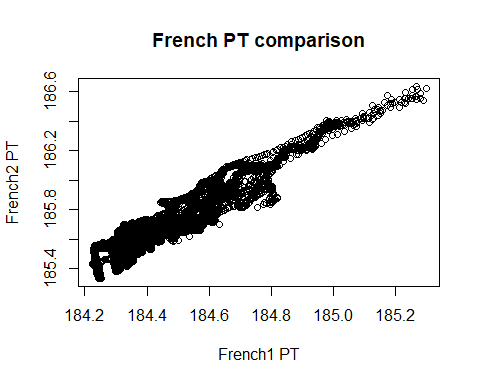
\includegraphics{Final_Q_files/figure-latex/unnamed-chunk-2-1.pdf} There
is a big increase in middle to end of may that doesnt seem to be real
from precip , and then a lot of vertical drops in middle of June, July,
August (potentially cleanning points) and then at the end of september
we get a big drop, this is when the site was taken out\ldots(PT was
taken out on the 21st)\ldots{} let the cleaning commence!

\hypertarget{moose-1.0}{%
\subsection{Moose 1.0}\label{moose-1.0}}

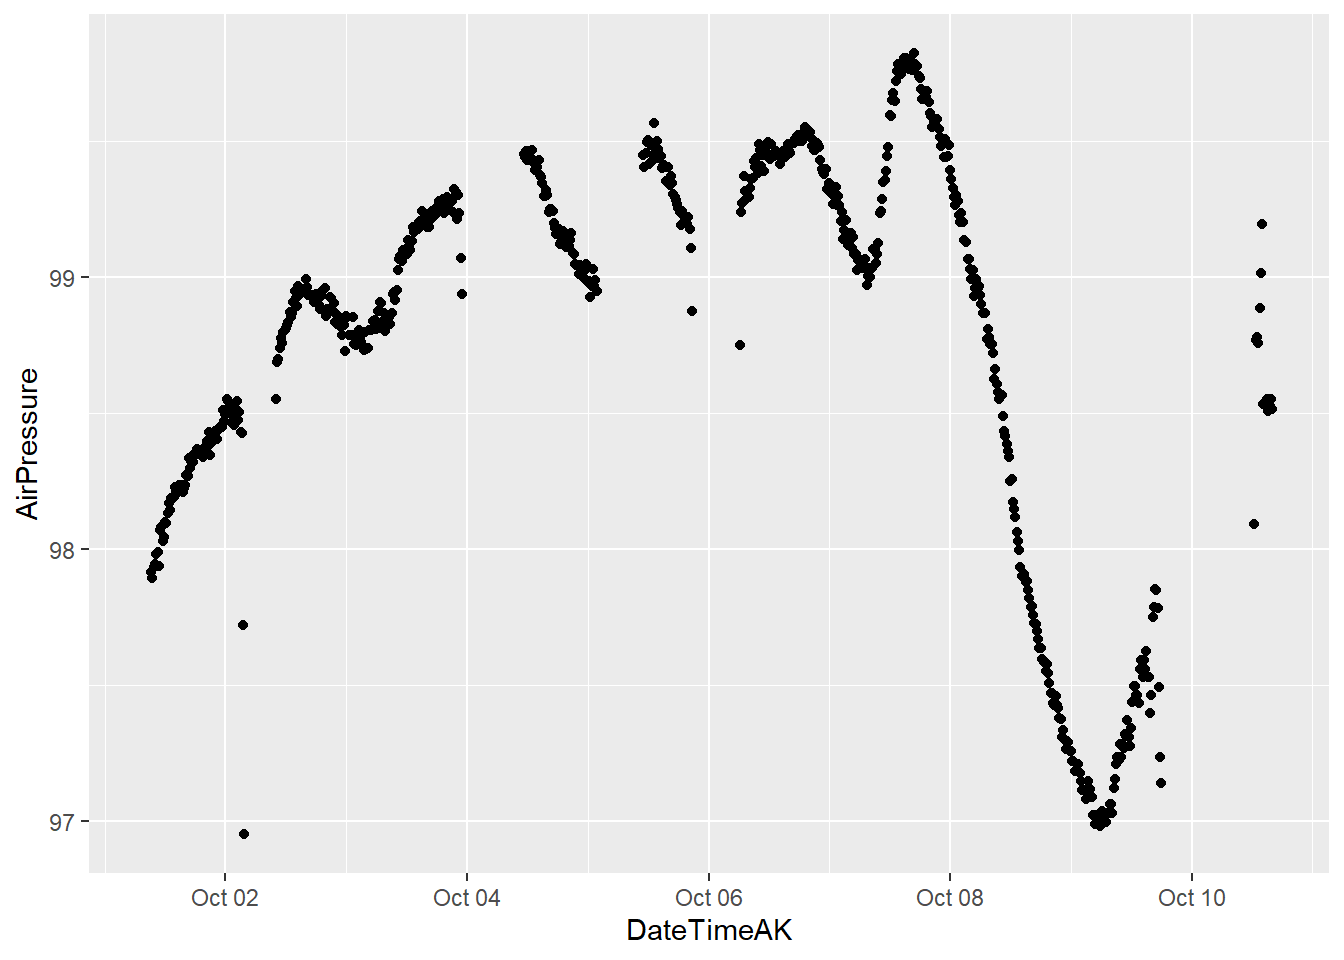
\includegraphics{Final_Q_files/figure-latex/unnamed-chunk-3-1.pdf}
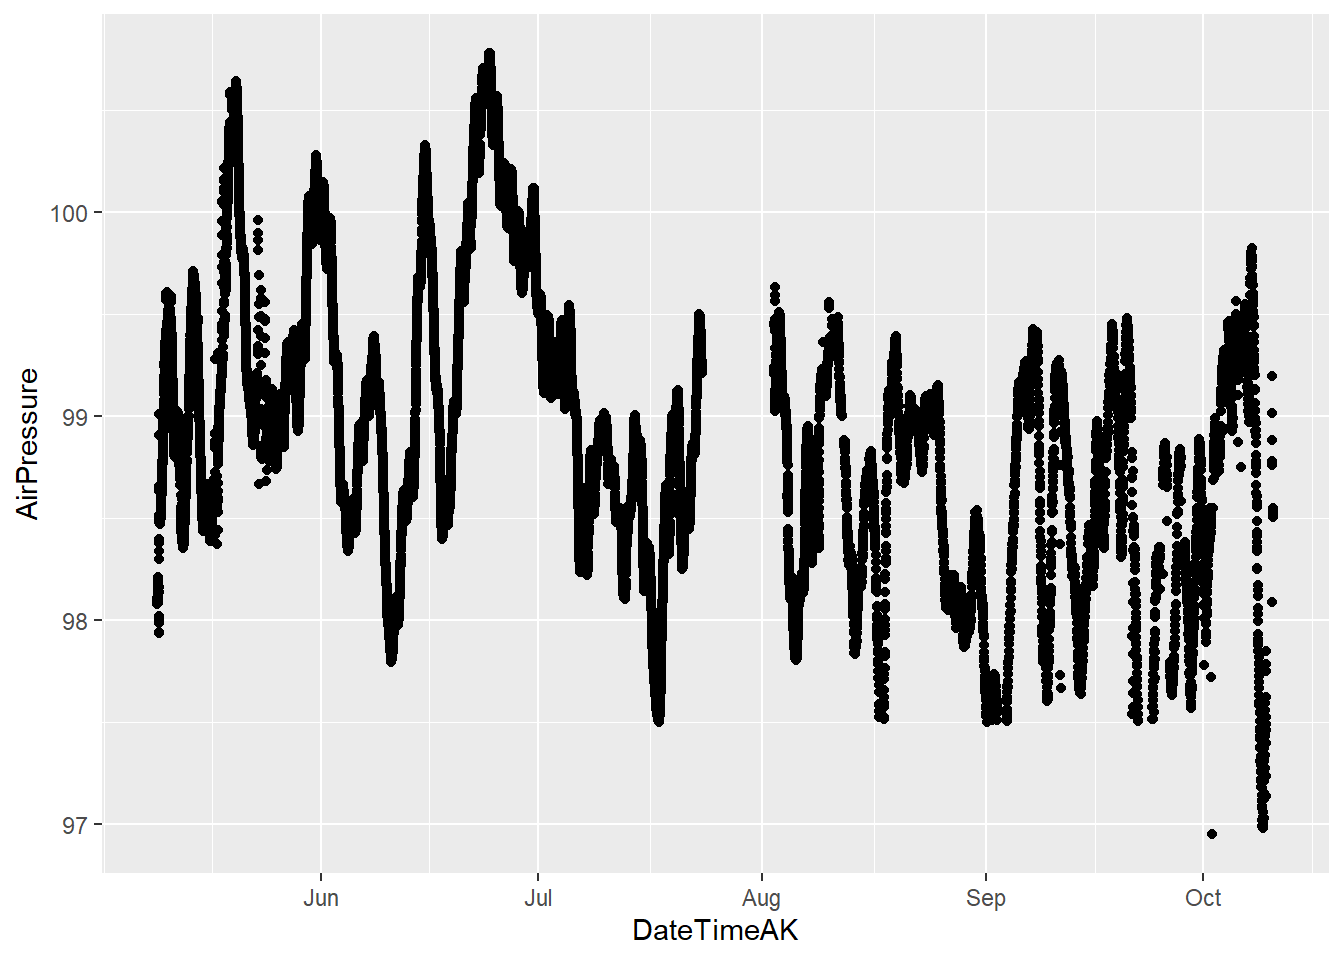
\includegraphics{Final_Q_files/figure-latex/unnamed-chunk-3-2.pdf}

\begin{verbatim}
## [1] 4052 5270 5271 5272 5273 5274 5275 5276 5277
\end{verbatim}

\includegraphics{Final_Q_files/figure-latex/unnamed-chunk-3-3.pdf}

\begin{verbatim}
## [1] 2047
\end{verbatim}

\includegraphics{Final_Q_files/figure-latex/unnamed-chunk-3-4.pdf}

\begin{verbatim}
## [1] 2679 2680 2681
\end{verbatim}

\includegraphics{Final_Q_files/figure-latex/unnamed-chunk-3-5.pdf}
\includegraphics{Final_Q_files/figure-latex/unnamed-chunk-3-6.pdf} 1)
Clipped off the take out date (anything after 2015-09-20 18:30:00) 2)
Set vertical drops in raw data to NA's 3) NEED TO DO NA INTERPRET

\hypertarget{impute-missing-observations-in-pressure-for-moose}{%
\subsubsection{Impute missing observations in pressure for
Moose}\label{impute-missing-observations-in-pressure-for-moose}}

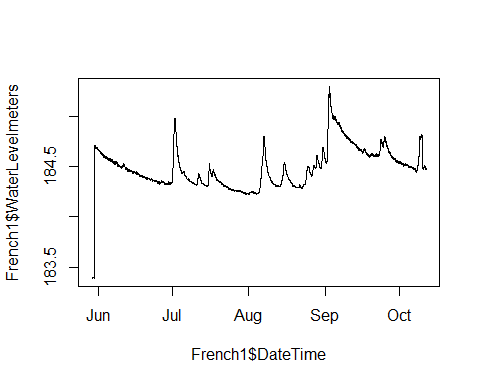
\includegraphics{Final_Q_files/figure-latex/unnamed-chunk-4-1.pdf} 1)
middle of July gap is just connected

\hypertarget{export-csv-to-dod_discharge-pt_data-2015}{%
\subsubsection{Export csv to
DoD\_Discharge-\textgreater PT\_data-\textgreater2015}\label{export-csv-to-dod_discharge-pt_data-2015}}

\hypertarget{raw-frch}{%
\subsection{Raw FRCH}\label{raw-frch}}

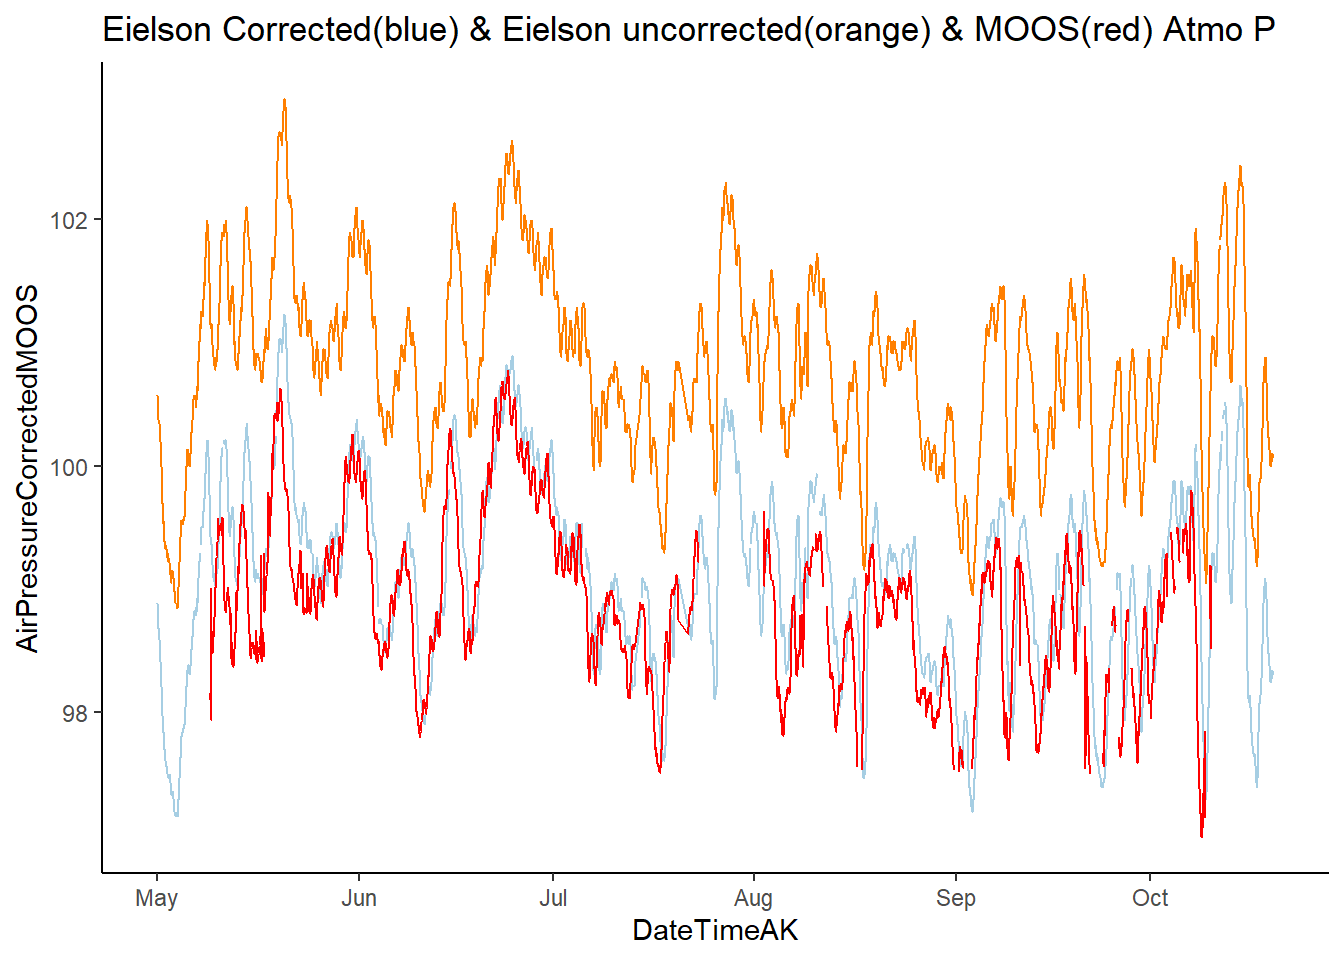
\includegraphics{Final_Q_files/figure-latex/unnamed-chunk-6-1.pdf}

Similarily to Moose There is a big increase in middle to end of may that
doesnt seem to be real from precip , and then a lot of vertical drops in
middle of June, July, August (potentially cleanning points) and then at
the end of september we get a big drop, this is when the site was taken
out\ldots(PT was taken out on the 21st)\ldots{} let the cleaning
commence!

\hypertarget{french-1.0}{%
\subsubsection{French 1.0}\label{french-1.0}}

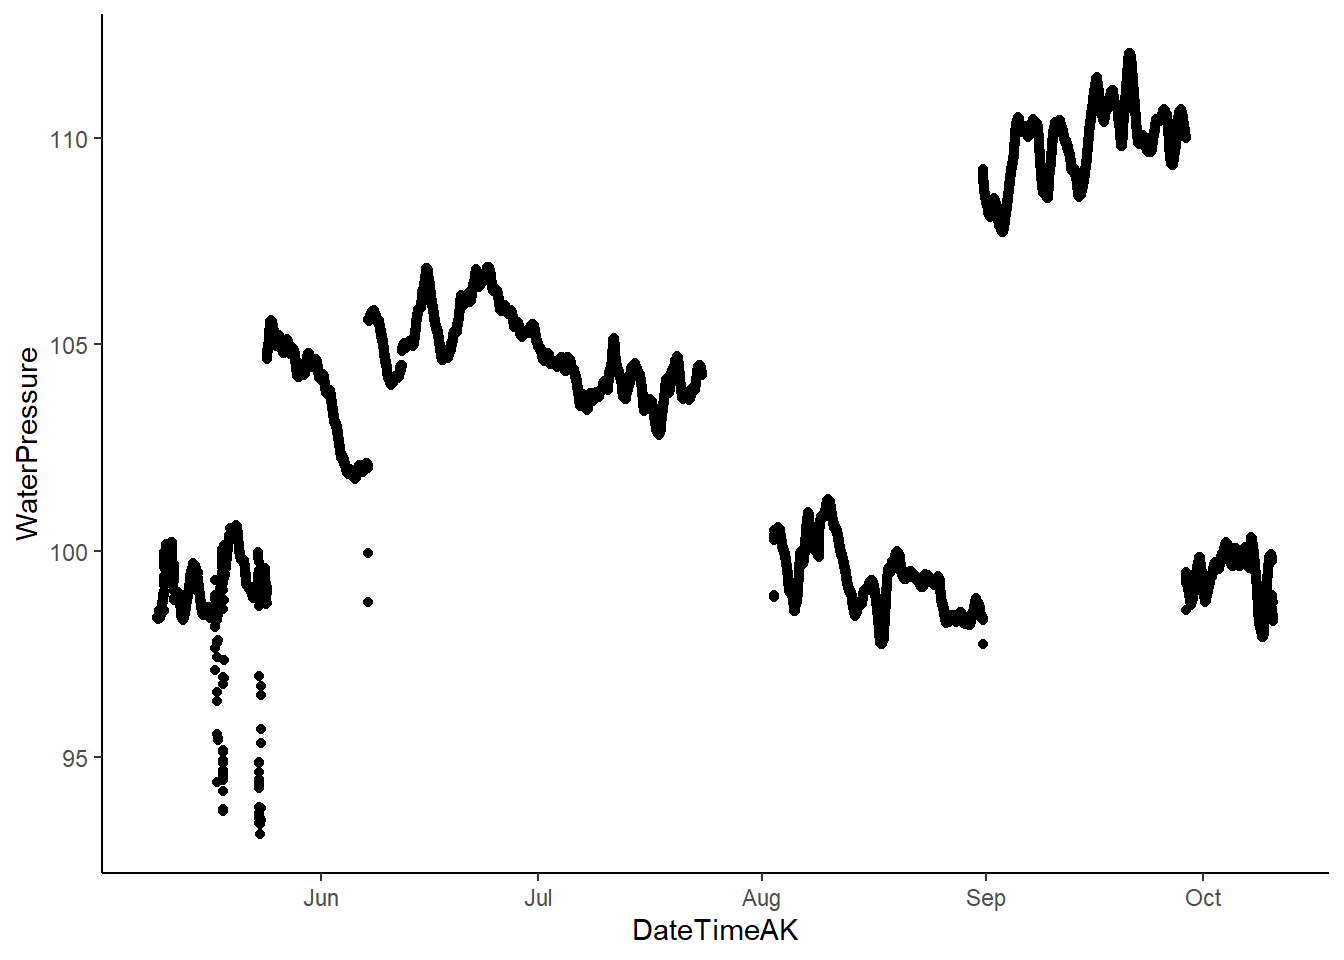
\includegraphics{Final_Q_files/figure-latex/unnamed-chunk-7-1.pdf}

\begin{verbatim}
##  [1] 1535 2047 2048 2049 2050 2051 2052 2053 2054 2055 2056 2057 2058 2059 2060
## [16] 3305 3306 3307 3308 3309 3310 3311 3312 3313 3314 3315 3316 3317 3318 3319
## [31] 3320 3321 3322 3323 3324 3325 3326 3327 3328 3329 3330 3331 3332 3333 3334
## [46] 3335 3336 3337 3338 3339 3340 3341 3342 3343 3344 3345 3346 3347 3348 3349
## [61] 3350 3351 3352 3353 3354 3355 3356 3357 3358 3359 3360 3361 3362 3363 3364
## [76] 3365 3366 3367 3368 3369 3370 3371 3372 3373 3374 3375 3376 3377 3378 3379
## [91] 3380 3381 3382 3383 3384
\end{verbatim}

\includegraphics{Final_Q_files/figure-latex/unnamed-chunk-7-2.pdf}

\begin{verbatim}
##  [1]   49 2052 5213 5214 5215 5216 5217 5218 5219 5220 5221 5222 5223 5224 5225
## [16] 5226 5227 5228 5229 5230 5231 5232 5233 5234 5235 5236 5237 5238 5239 5240
## [31] 5241
\end{verbatim}

\includegraphics{Final_Q_files/figure-latex/unnamed-chunk-7-3.pdf}
\includegraphics{Final_Q_files/figure-latex/unnamed-chunk-7-4.pdf}

\begin{verbatim}
##  [1] 2641 2642 2643 2644 2645 2646 2647 2648 2649 2650 2651 2652 2653 2654 2655
## [16] 2656 4631 4632 4633 4654
\end{verbatim}

\includegraphics{Final_Q_files/figure-latex/unnamed-chunk-7-5.pdf}
\includegraphics{Final_Q_files/figure-latex/unnamed-chunk-7-6.pdf} 1)
Clipped off the take out date (anything after 2015-09-20 18:30:00) 2)
Set vertical drops in raw data to NA's 3) NEED TO DO NA INTERPRET
(na\_kalman)

\hypertarget{impute-missing-observations-in-pressure-for-moose-1}{%
\subsubsection{Impute missing observations in pressure for
Moose}\label{impute-missing-observations-in-pressure-for-moose-1}}

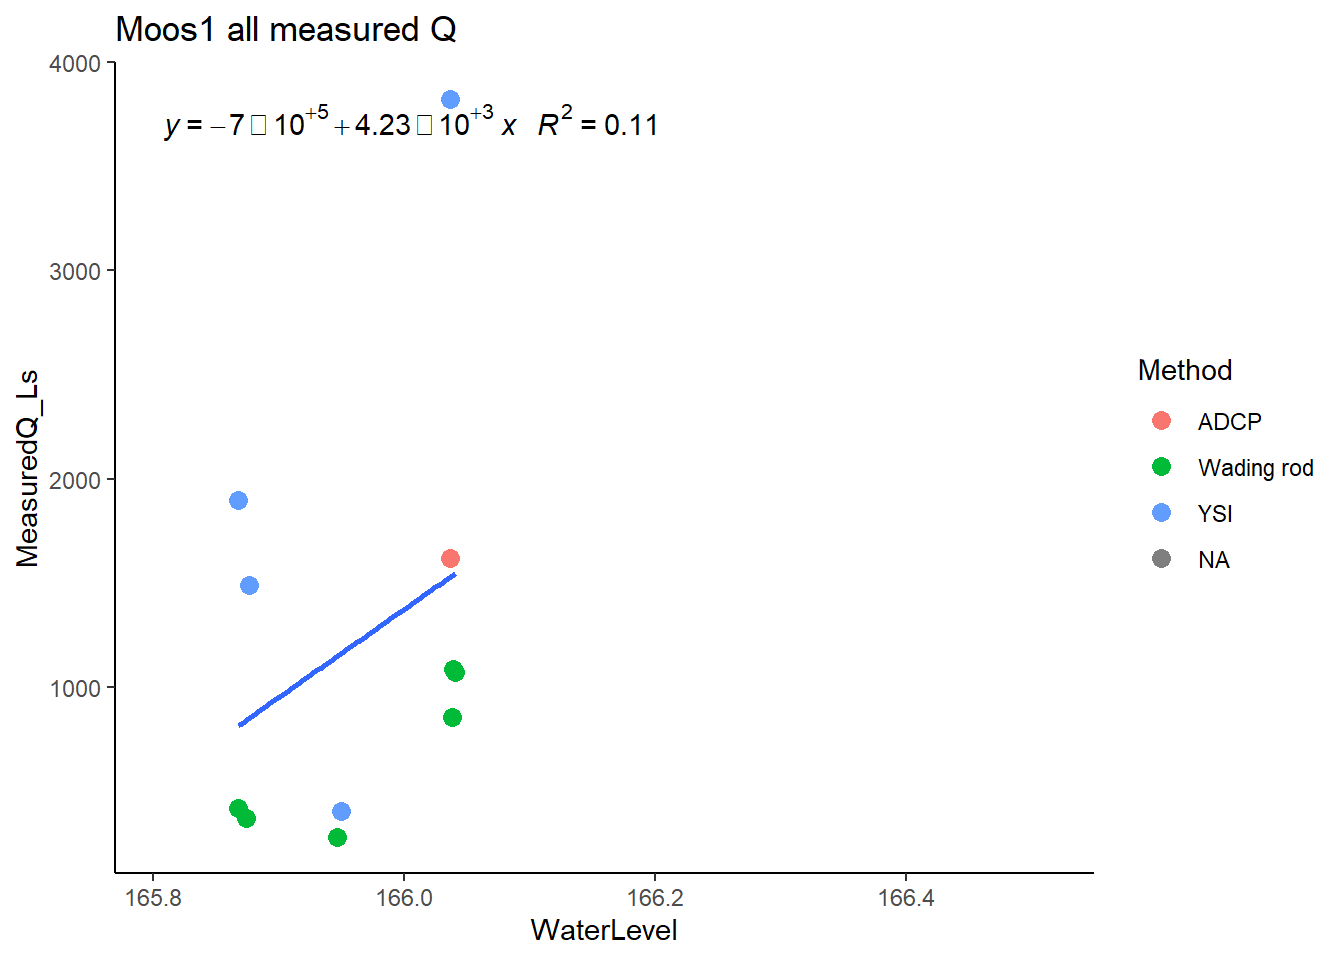
\includegraphics{Final_Q_files/figure-latex/unnamed-chunk-8-1.pdf}

\hypertarget{export-csv-to-dod_discharge-pt_data-2015-1}{%
\subsubsection{Export csv to
DoD\_Discharge-\textgreater PT\_data-\textgreater2015}\label{export-csv-to-dod_discharge-pt_data-2015-1}}

\hypertarget{observed-discharge-at-french-and-moose}{%
\subsubsection{Observed Discharge at French and
Moose}\label{observed-discharge-at-french-and-moose}}

Slugs were the only method of discharge for 2015

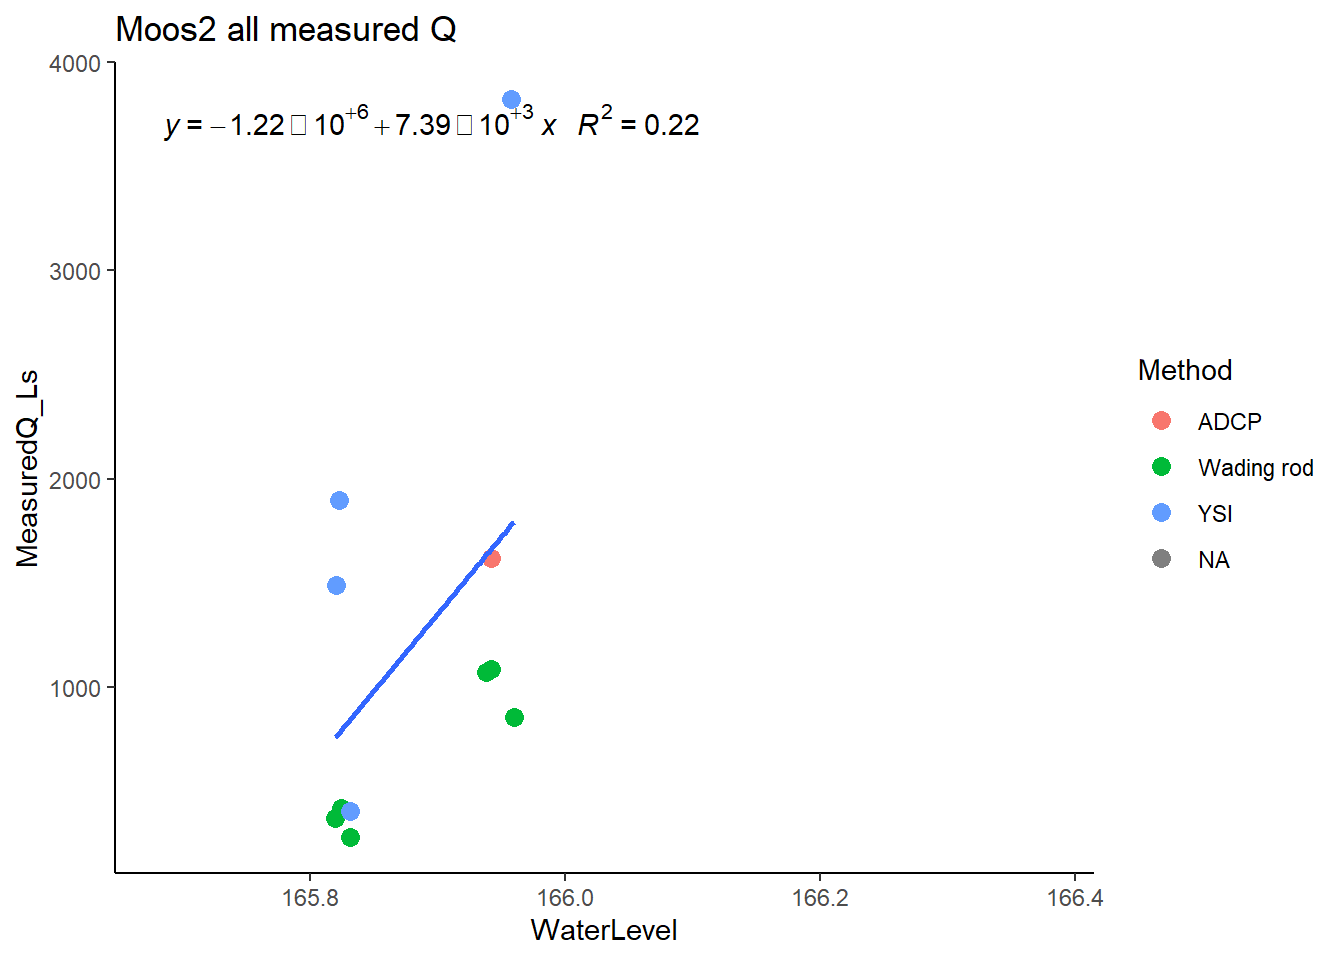
\includegraphics{Final_Q_files/figure-latex/unnamed-chunk-10-1.pdf}
\includegraphics{Final_Q_files/figure-latex/unnamed-chunk-10-2.pdf}
\includegraphics{Final_Q_files/figure-latex/unnamed-chunk-10-3.pdf}
\includegraphics{Final_Q_files/figure-latex/unnamed-chunk-10-4.pdf} This
is from the DOD Q Summary csv that is DoD Project-\textgreater2015 AK
sensors -\textgreater Discharge

\hypertarget{raw-rating-curve-with-moose-1-pressure-transducer}{%
\subsubsection{Raw Rating Curve with Moose 1 Pressure
Transducer}\label{raw-rating-curve-with-moose-1-pressure-transducer}}

\begin{verbatim}
## Joining, by = c("DateTime", "site")
\end{verbatim}

\begin{verbatim}
## `geom_smooth()` using formula 'y ~ x'
\end{verbatim}

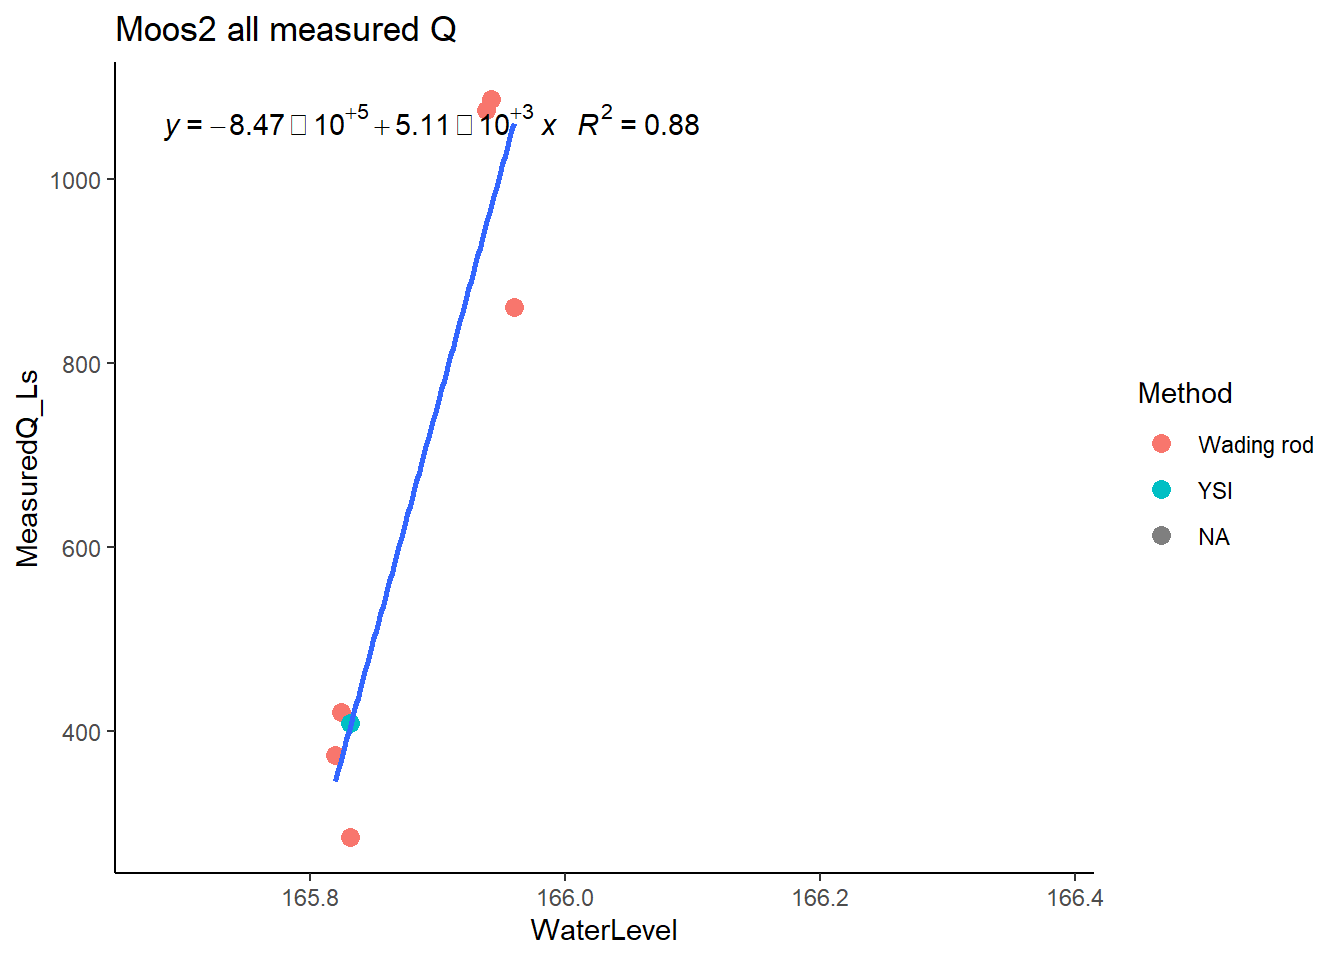
\includegraphics{Final_Q_files/figure-latex/unnamed-chunk-11-1.pdf} The
most upper measurement is probably bad. I am going to take it out

\hypertarget{rating-curve-with-moose-1-pressure-transducer-2.0}{%
\subsubsection{Rating Curve with Moose 1 Pressure Transducer
2.0}\label{rating-curve-with-moose-1-pressure-transducer-2.0}}

\begin{verbatim}
## Joining, by = c("DateTime", "site")
\end{verbatim}

\begin{verbatim}
## `geom_smooth()` using formula 'y ~ x'
\end{verbatim}

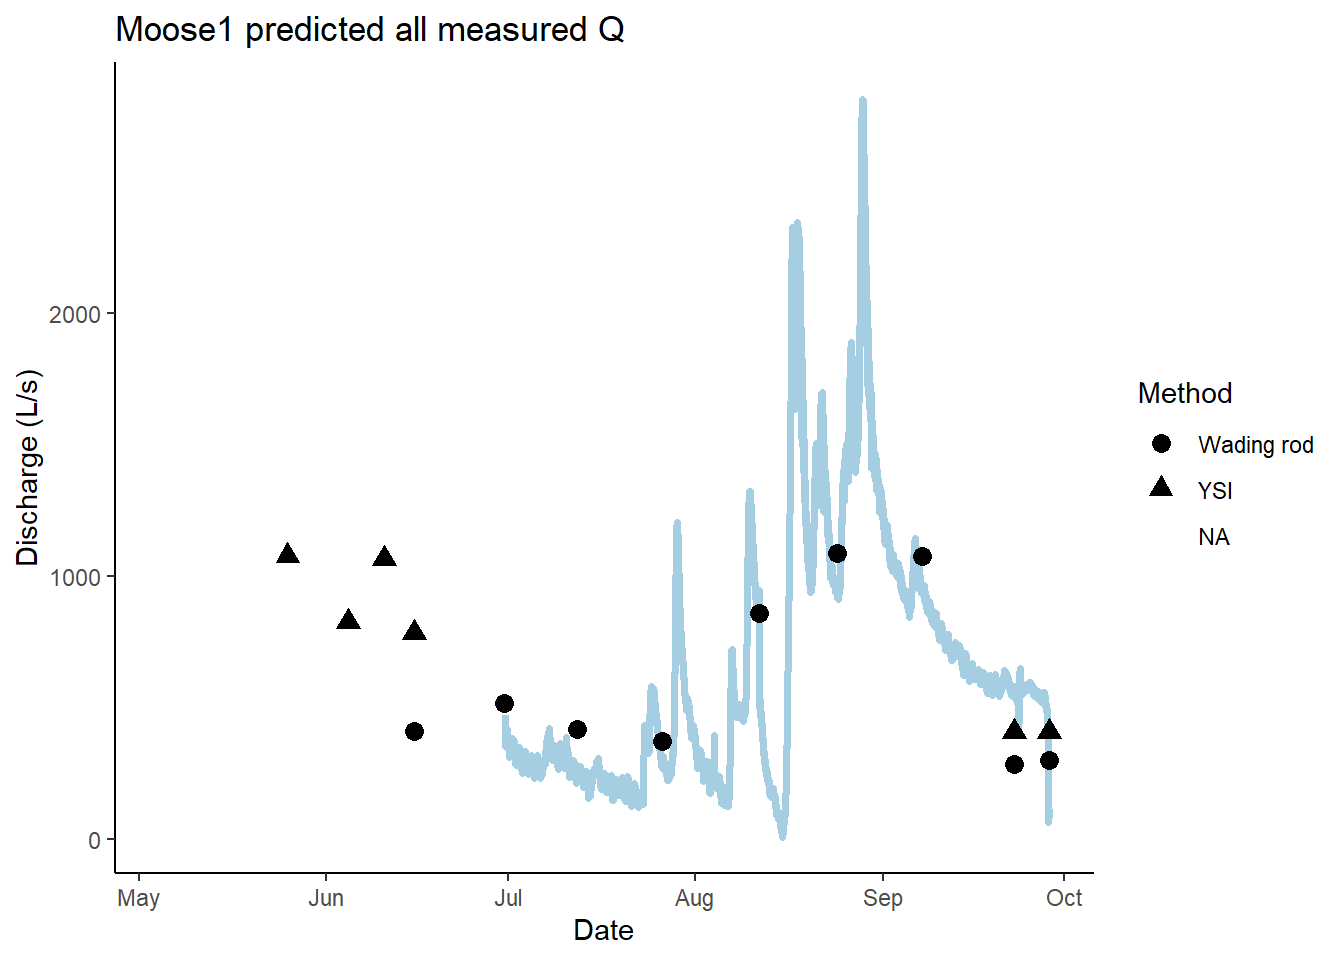
\includegraphics{Final_Q_files/figure-latex/unnamed-chunk-12-1.pdf}

\begin{verbatim}
## Joining, by = c("DateTime", "site")
## `geom_smooth()` using formula 'y ~ x'
\end{verbatim}

\includegraphics{Final_Q_files/figure-latex/unnamed-chunk-12-2.pdf}

\begin{verbatim}
## `geom_smooth()` using formula 'y ~ x'
## `geom_smooth()` using formula 'y ~ x'
## `geom_smooth()` using formula 'y ~ x'
\end{verbatim}

\includegraphics{Final_Q_files/figure-latex/unnamed-chunk-12-3.pdf} 1)
Removed the point that had a Q \textgreater{} 3000 L/s - This R\^{}2
value is actually lower 2) Removed the point that had a Q \textgreater{}
1300 L/s - best R\^{}2 value

\hypertarget{moose1-light-blue-and-moose2-and-moose3-brown-with-observed-q.}{%
\subsubsection{Moose1 (light blue) and Moose2 and Moose3 (brown) with
observed
Q.}\label{moose1-light-blue-and-moose2-and-moose3-brown-with-observed-q.}}

\hypertarget{black-points-are-observed-q}{%
\paragraph{Black points are observed
Q}\label{black-points-are-observed-q}}

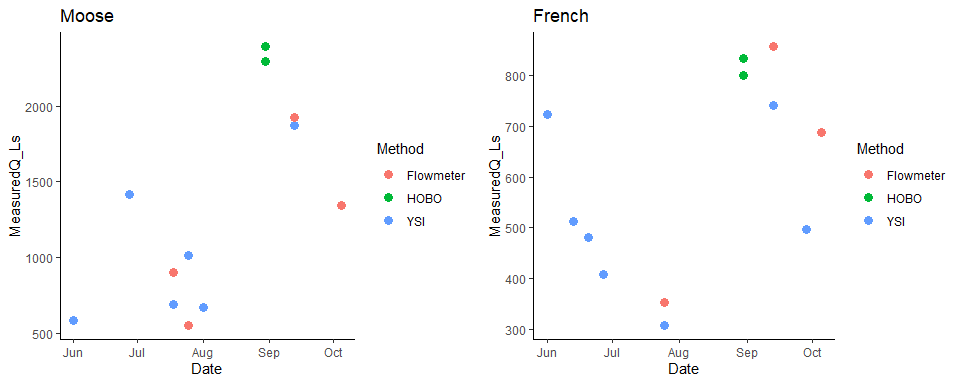
\includegraphics{Final_Q_files/figure-latex/unnamed-chunk-13-1.pdf}
\includegraphics{Final_Q_files/figure-latex/unnamed-chunk-13-2.pdf}
\includegraphics{Final_Q_files/figure-latex/unnamed-chunk-13-3.pdf}
\includegraphics{Final_Q_files/figure-latex/unnamed-chunk-13-4.pdf} This
is only from PT rather than waterlevel, is that going to be a problem?
Moose1 is from the first RC and Moose2 is from the second RC and Moose3
is from the third RC. It appears that it gets worse to predict the
higher discharges as we go through our iteration of RC's.

\hypertarget{export-csv-to-dod_discharge-pt_data-2015-2}{%
\subsubsection{Export csv to
DoD\_Discharge-\textgreater PT\_data-\textgreater2015}\label{export-csv-to-dod_discharge-pt_data-2015-2}}

\hypertarget{raw-rating-curve-with-french-1-pressure-transducer}{%
\subsubsection{Raw Rating Curve with French 1 Pressure
Transducer}\label{raw-rating-curve-with-french-1-pressure-transducer}}

\begin{verbatim}
## Joining, by = c("DateTime", "site")
\end{verbatim}

\begin{verbatim}
## `geom_smooth()` using formula 'y ~ x'
\end{verbatim}

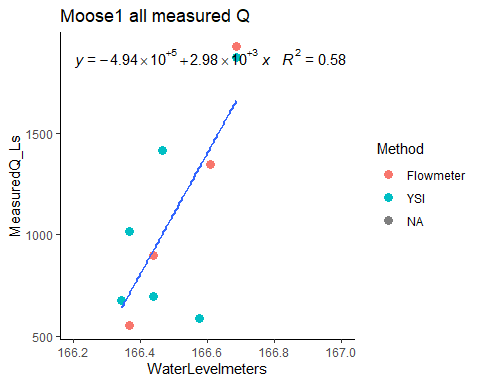
\includegraphics{Final_Q_files/figure-latex/unnamed-chunk-15-1.pdf} The
most upper measurement is probably bad. I am going to take it out

\hypertarget{rating-curve-french-pt-2.0}{%
\subsubsection{Rating Curve French PT
2.0}\label{rating-curve-french-pt-2.0}}

\begin{verbatim}
## Joining, by = c("DateTime", "site")
\end{verbatim}

\begin{verbatim}
## `geom_smooth()` using formula 'y ~ x'
\end{verbatim}

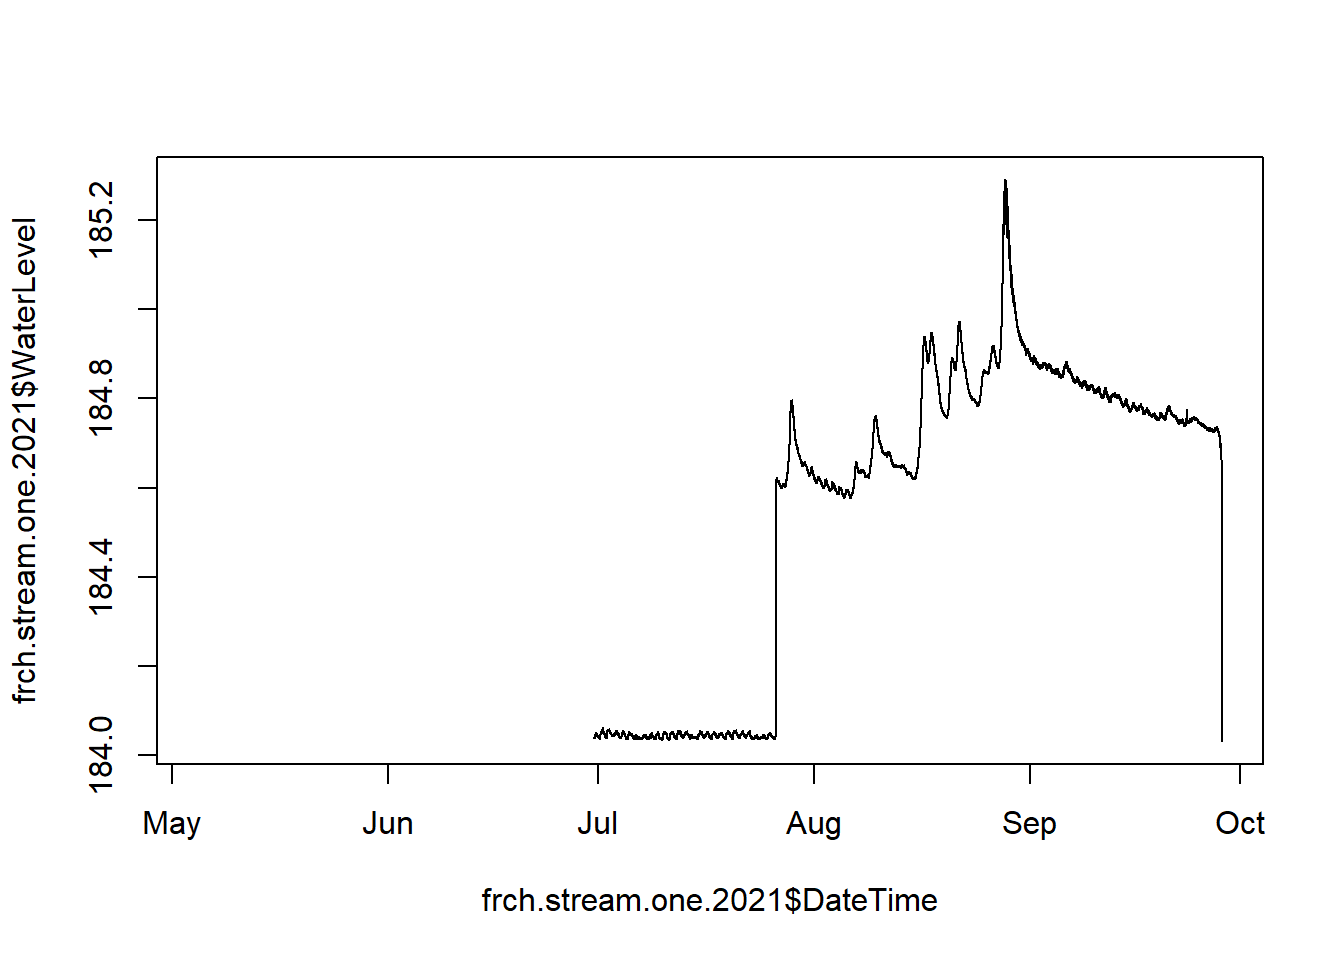
\includegraphics{Final_Q_files/figure-latex/unnamed-chunk-16-1.pdf}
R\^{}2 value goes down

\hypertarget{french-1-calculated-q-ls}{%
\subsection{French 1 Calculated Q
(L/s)}\label{french-1-calculated-q-ls}}

\hypertarget{black-points-are-observed-q-1}{%
\paragraph{Black points are observed
Q}\label{black-points-are-observed-q-1}}

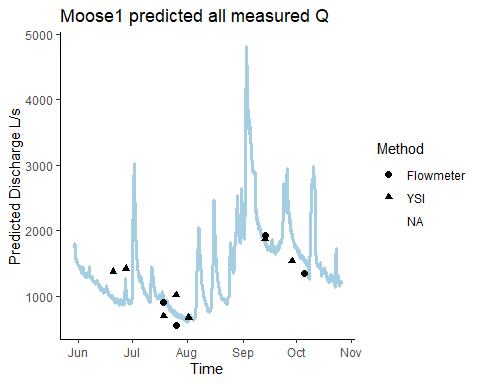
\includegraphics{Final_Q_files/figure-latex/unnamed-chunk-17-1.pdf} This
is not great considering there are negative values

\hypertarget{export-csv-to-dod_discharge-pt_data-2015-3}{%
\subsubsection{Export csv to
DoD\_Discharge-\textgreater PT\_data-\textgreater2015}\label{export-csv-to-dod_discharge-pt_data-2015-3}}

\hypertarget{export-csv-to-dod_discharge-pt_data-2015-4}{%
\subsubsection{Export csv to
DoD\_Discharge-\textgreater PT\_data-\textgreater2015}\label{export-csv-to-dod_discharge-pt_data-2015-4}}

\hypertarget{french-and-moose-2018-discharge}{%
\section{French and Moose 2018
Discharge}\label{french-and-moose-2018-discharge}}

2018 data is read from DoD-\textgreater2018 sesors French
Moose-\textgreater Q-\textgreater Qprocessing-\textgreater{}``French\_stream\_PT\_may-oct2018\_20005933.csv''
Wading rods and slugs were used to measure discrete Q during site visit

\hypertarget{checking-closeness-between-the-two-pressure-transducers}{%
\subparagraph{Checking closeness between the two Pressure
Transducers}\label{checking-closeness-between-the-two-pressure-transducers}}

1:1 line in green
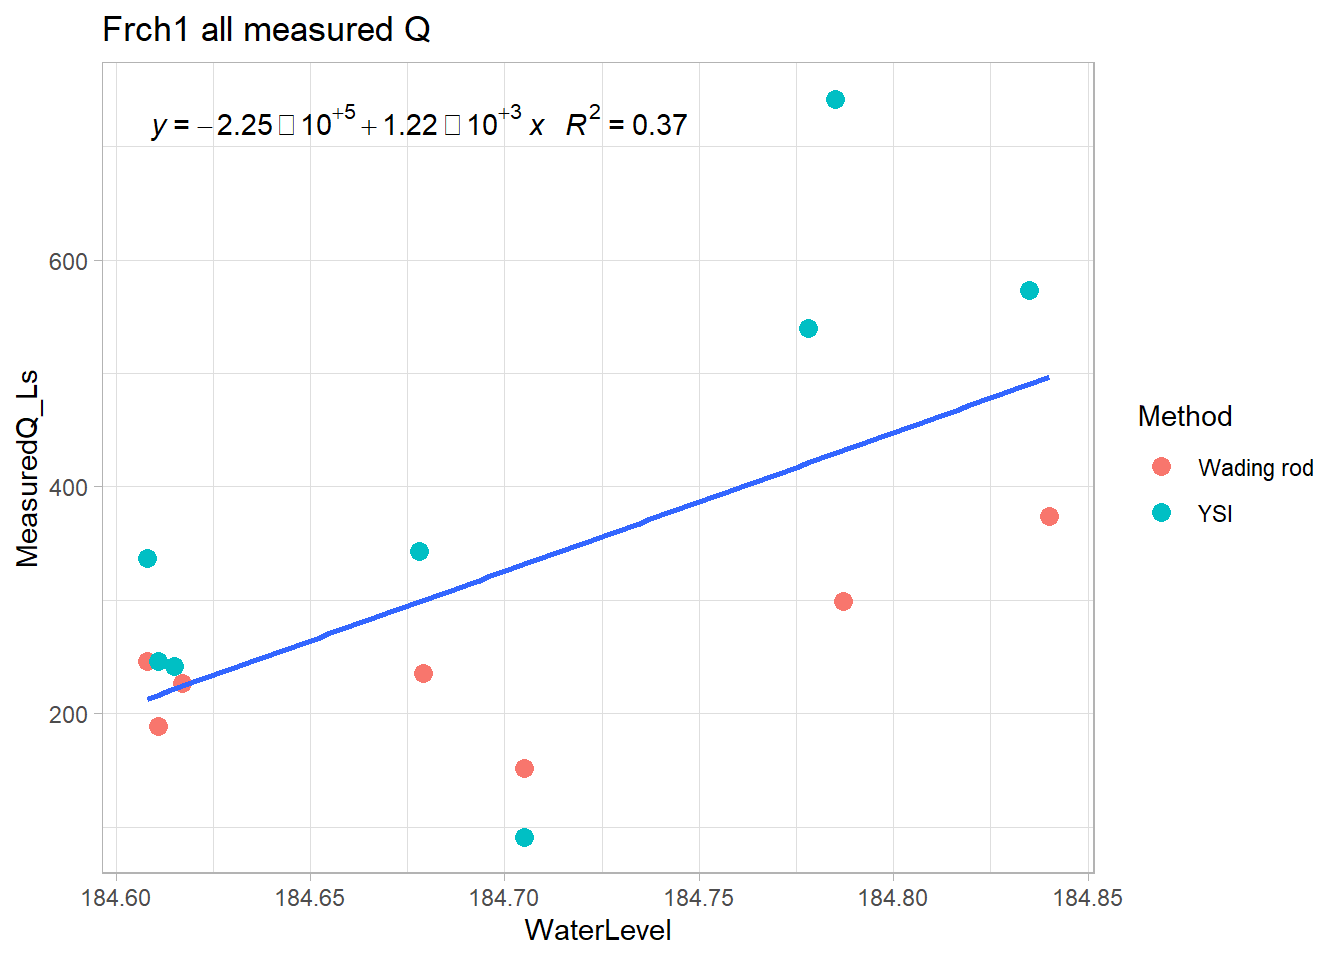
\includegraphics{Final_Q_files/figure-latex/unnamed-chunk-21-1.pdf}
\includegraphics{Final_Q_files/figure-latex/unnamed-chunk-21-2.pdf}

\hypertarget{french}{%
\subsubsection{French}\label{french}}

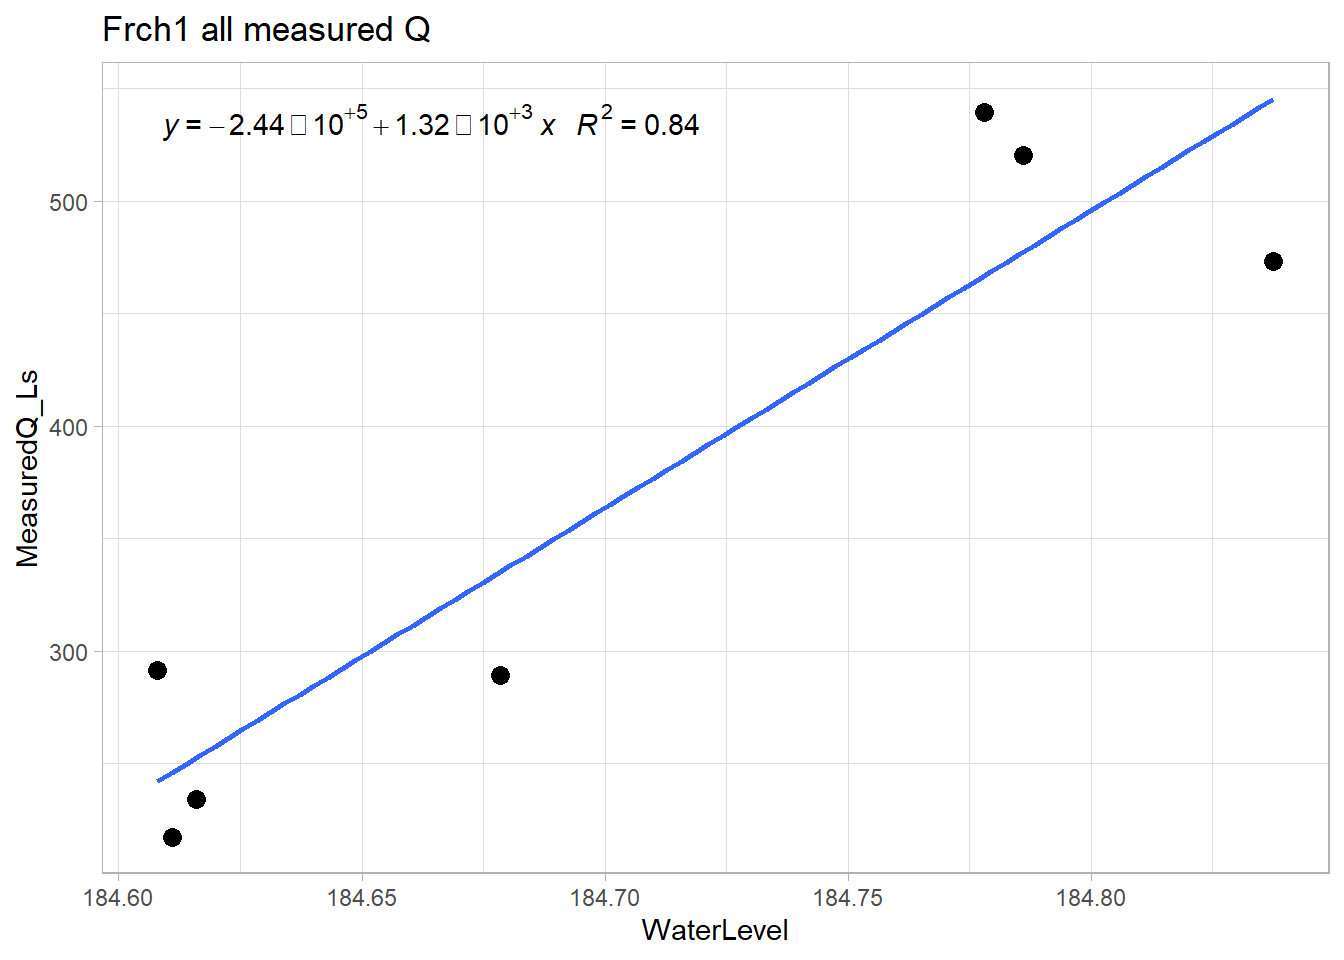
\includegraphics{Final_Q_files/figure-latex/unnamed-chunk-22-1.pdf}
There looks like an error when we calculated depth. Tom says that we can
adjust the difference of the wrong one to make them agree, then
remeasure them next year. French 2 also looks ``noisier'' 1) dumping
French 2

\hypertarget{raw-french-1}{%
\subsubsection{Raw French 1}\label{raw-french-1}}

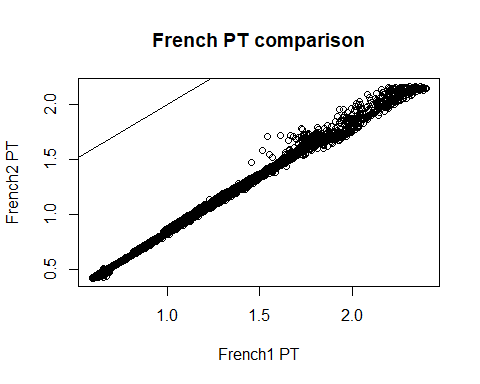
\includegraphics{Final_Q_files/figure-latex/unnamed-chunk-23-1.pdf} The
beginning is probably when this was installed, I will remove that. the
spije in October is confirmed with French 2 so that is real. let the
cleaning commence!

\hypertarget{french-pt-1-2.0}{%
\subsubsection{French PT 1 2.0}\label{french-pt-1-2.0}}

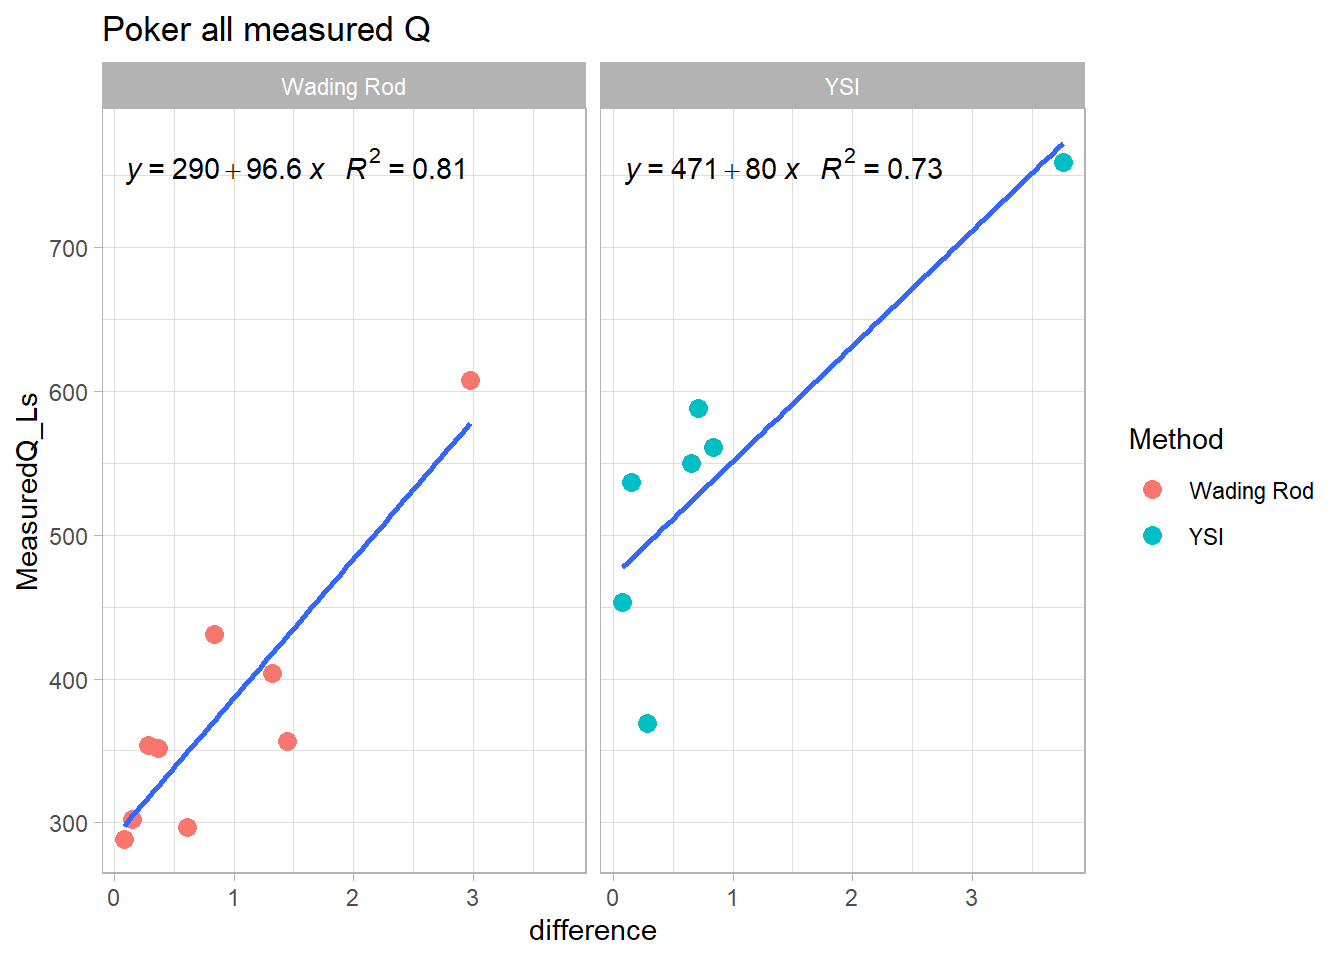
\includegraphics{Final_Q_files/figure-latex/unnamed-chunk-24-1.pdf} 1)
set the beginning of the dataframe where PT was taking out of water
points to NA 2) we are dumping French PT2 due to it being too ``noisy''

\hypertarget{export-pt-data-to-csv-to-dod_discharge-pt_data-2018}{%
\subsubsection{export PT data to csv to
DoD\_Discharge-\textgreater PT\_data-\textgreater2018}\label{export-pt-data-to-csv-to-dod_discharge-pt_data-2018}}

\hypertarget{raw-moose-1}{%
\subsubsection{Raw Moose}\label{raw-moose-1}}

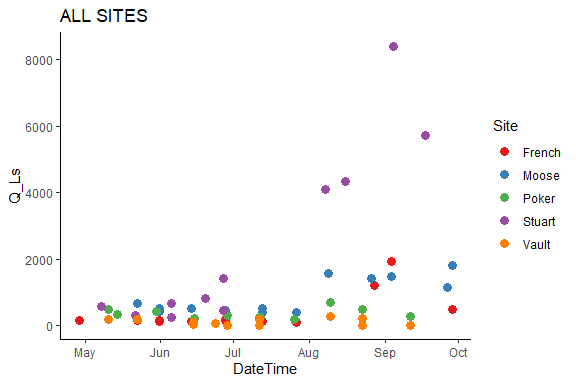
\includegraphics{Final_Q_files/figure-latex/unnamed-chunk-26-1.pdf}
Moose2 looks a little weird during mid July, where it doens't agree w/
Moose 1. Moose 2 seems a lot noisier\ldots.we are dumping moose 2

\hypertarget{moose-pt-1-2.0}{%
\subsubsection{Moose PT 1 2.0}\label{moose-pt-1-2.0}}

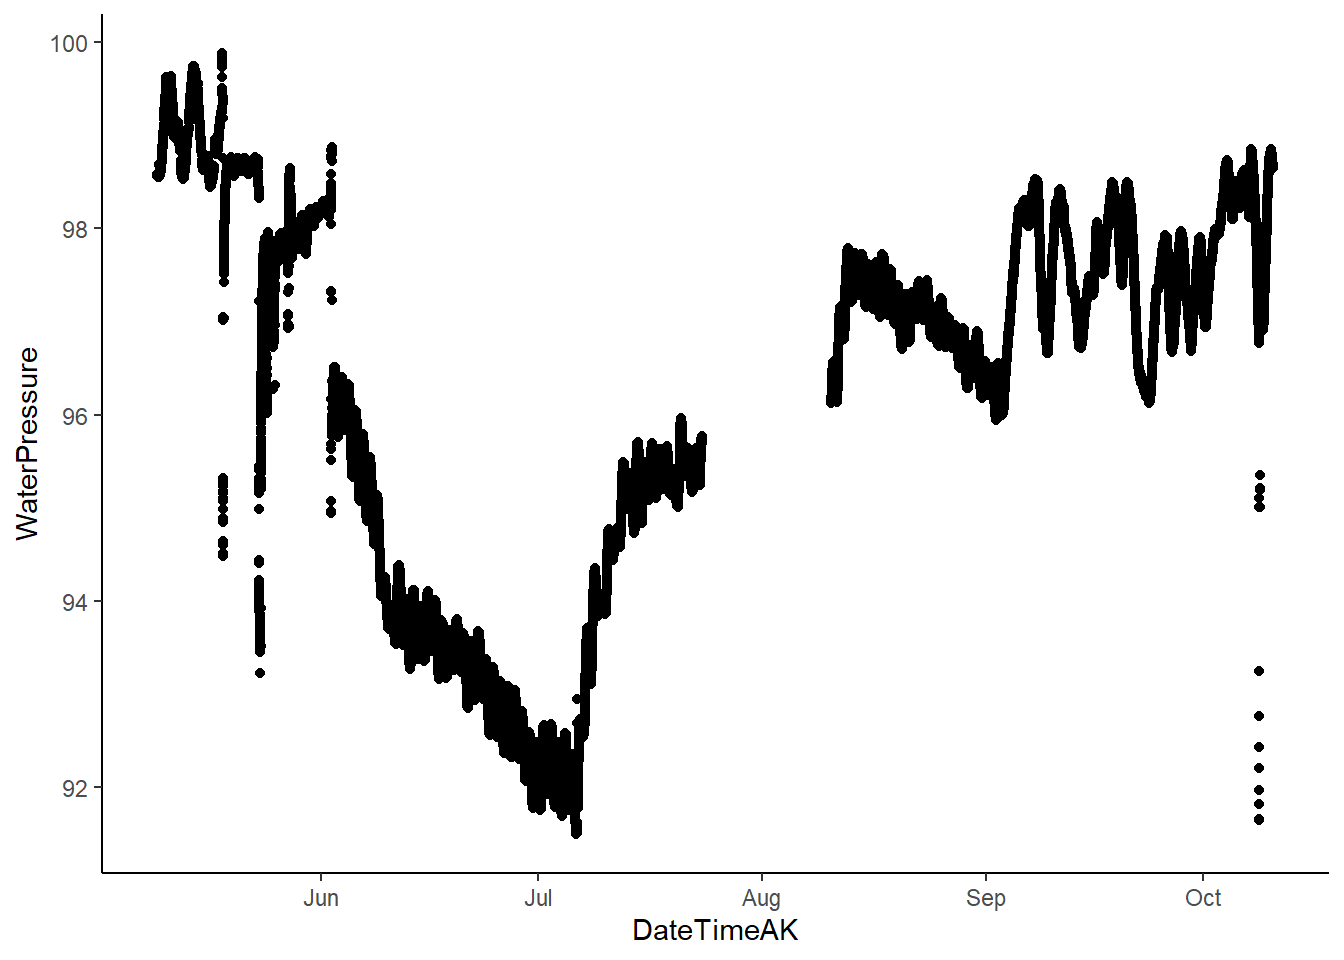
\includegraphics{Final_Q_files/figure-latex/unnamed-chunk-27-1.pdf}
\includegraphics{Final_Q_files/figure-latex/unnamed-chunk-27-2.pdf} 1)
Removed the beginning and end of the dataframe where the PT was out of
water 2) Cleaned the receding limb of the september storm and replaced
it with the receding limb from the second PT however now we get a steep
drop for the end of the timeseries. Should I shift the back half of the
dataframe up? 3) set middle of Setember vertical drop to NAs 4) still
need to do NA INTERPRET!

\hypertarget{impute-missing-observations-in-pressure-for-moos}{%
\subsubsection{Impute missing observations in pressure for
MOOS}\label{impute-missing-observations-in-pressure-for-moos}}

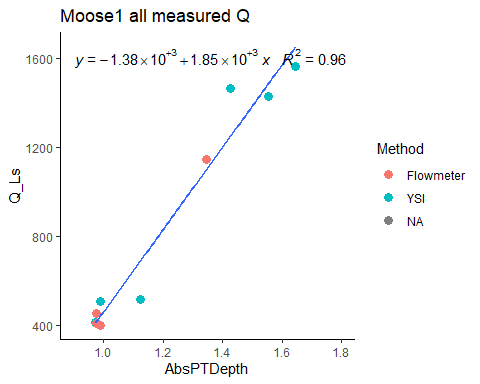
\includegraphics{Final_Q_files/figure-latex/unnamed-chunk-28-1.pdf}
\#\#\# Observed Discharge at French and Moose

\begin{itemize}
\tightlist
\item
  from Rachel Voight For the days we used the HOBO, there are two
  ``measurements'' since I did not know which slug solution was used, so
  I calculated it with the two likely slug batches. We changed where we
  were measuring Q at Moose; the first two times we measured Q, we did
  it downstream of the sensors near the actual pressure transducer. We
  likely underestimated Q for those few measurements at the old spot
  downstream of the sensors.
\end{itemize}

\hypertarget{export-pt-data-to-csv-to-dod_discharge-pt_data-2018-1}{%
\subsubsection{export PT data to csv to
DoD\_Discharge-\textgreater PT\_data-\textgreater2018}\label{export-pt-data-to-csv-to-dod_discharge-pt_data-2018-1}}

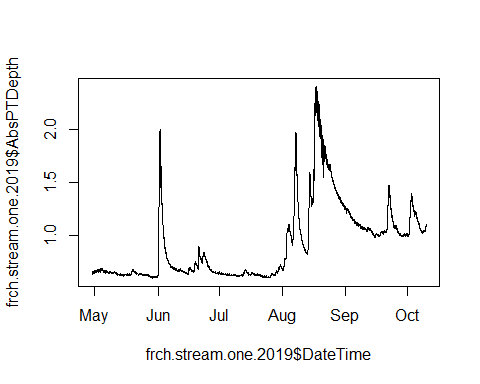
\includegraphics{Final_Q_files/figure-latex/unnamed-chunk-30-1.pdf}

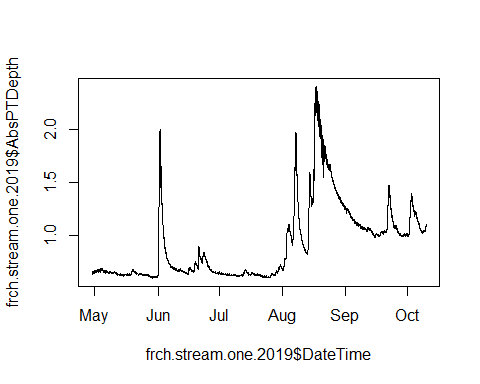
\includegraphics{Final_Q_files/figure-latex/unnamed-chunk-31-1.pdf}

\hypertarget{raw-rating-curve-with-moose-1-pressure-transducer-1}{%
\subsubsection{Raw Rating Curve with Moose 1 Pressure
Transducer}\label{raw-rating-curve-with-moose-1-pressure-transducer-1}}

\begin{verbatim}
## Joining, by = "DateTime"
\end{verbatim}

\begin{verbatim}
## `geom_smooth()` using formula 'y ~ x'
\end{verbatim}

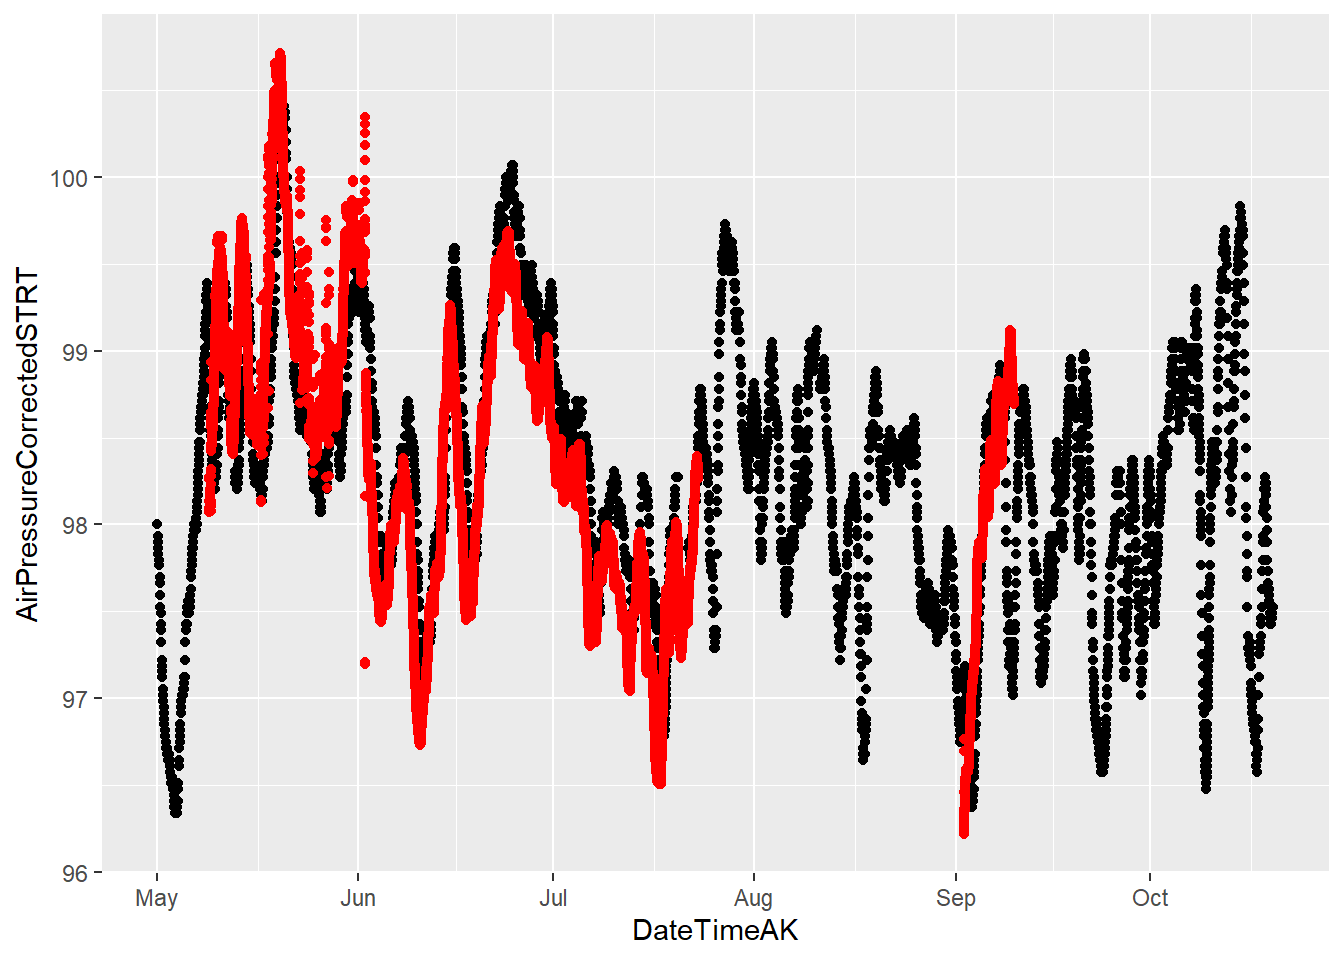
\includegraphics{Final_Q_files/figure-latex/unnamed-chunk-32-1.pdf}

\begin{verbatim}
## 
## Call:
## lm(formula = moose1comb$MeasuredQ_Ls ~ moose1comb$WaterLevelmeters)
## 
## Residuals:
##     Min      1Q  Median      3Q     Max 
## -892.01 -137.60  -13.08  328.47  414.47 
## 
## Coefficients:
##                              Estimate Std. Error t value Pr(>|t|)    
## (Intercept)                 -655003.6   134968.0  -4.853 0.000668 ***
## moose1comb$WaterLevelmeters    3941.1      810.5   4.863 0.000659 ***
## ---
## Signif. codes:  0 '***' 0.001 '**' 0.01 '*' 0.05 '.' 0.1 ' ' 1
## 
## Residual standard error: 385.2 on 10 degrees of freedom
##   (7193 observations deleted due to missingness)
## Multiple R-squared:  0.7028, Adjusted R-squared:  0.6731 
## F-statistic: 23.65 on 1 and 10 DF,  p-value: 0.0006587
\end{verbatim}

\begin{itemize}
\tightlist
\item
  Rachel -While we only had 4 measurements from the flow meter, they
  agree well with our trendline and slug Q. *Jake - I will remove the
  Hobo points in this regression
\end{itemize}

\begin{verbatim}
## Joining, by = "DateTime"
\end{verbatim}

\begin{verbatim}
## `geom_smooth()` using formula 'y ~ x'
\end{verbatim}

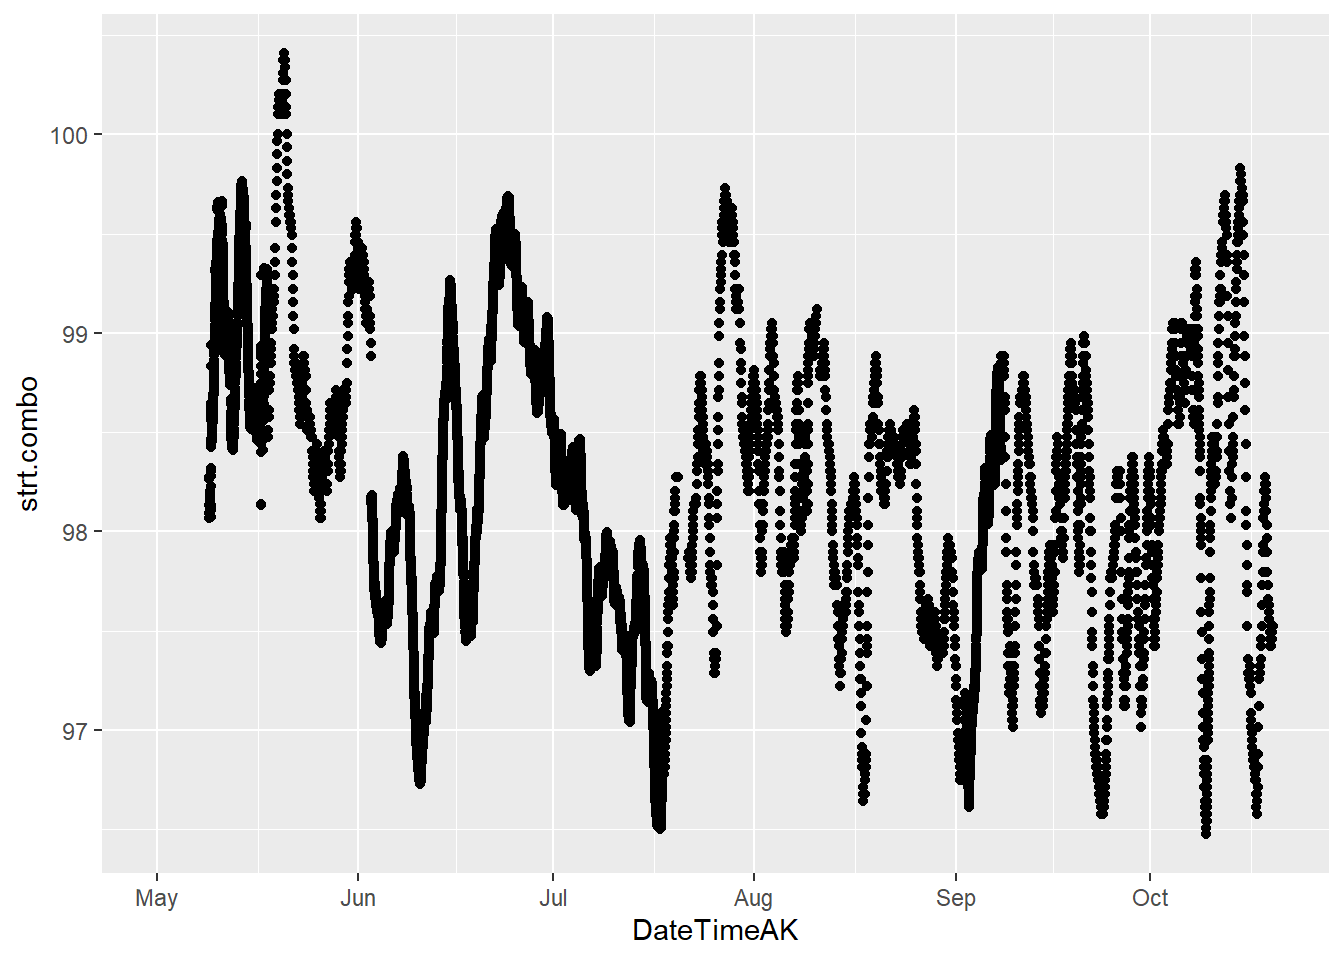
\includegraphics{Final_Q_files/figure-latex/unnamed-chunk-33-1.pdf}

\begin{verbatim}
## 
## Call:
## lm(formula = moose2comb$MeasuredQ_Ls ~ moose2comb$WaterLevelmeters)
## 
## Residuals:
##     Min      1Q  Median      3Q     Max 
## -743.40 -137.13    7.04  251.46  410.44 
## 
## Coefficients:
##                              Estimate Std. Error t value Pr(>|t|)  
## (Intercept)                 -494491.1   150037.5  -3.296   0.0109 *
## moose2comb$WaterLevelmeters    2976.6      901.1   3.303   0.0108 *
## ---
## Signif. codes:  0 '***' 0.001 '**' 0.01 '*' 0.05 '.' 0.1 ' ' 1
## 
## Residual standard error: 355.7 on 8 degrees of freedom
##   (7194 observations deleted due to missingness)
## Multiple R-squared:  0.577,  Adjusted R-squared:  0.5241 
## F-statistic: 10.91 on 1 and 8 DF,  p-value: 0.01081
\end{verbatim}

\begin{enumerate}
\def\labelenumi{\arabic{enumi})}
\tightlist
\item
  removed the HOBO ware points
\end{enumerate}

\hypertarget{estimated-q-from-moose-1-pt.}{%
\subsection{Estimated Q from Moose 1
PT.}\label{estimated-q-from-moose-1-pt.}}

\hypertarget{black-points-are-observed-q-2}{%
\paragraph{Black points are observed
Q}\label{black-points-are-observed-q-2}}

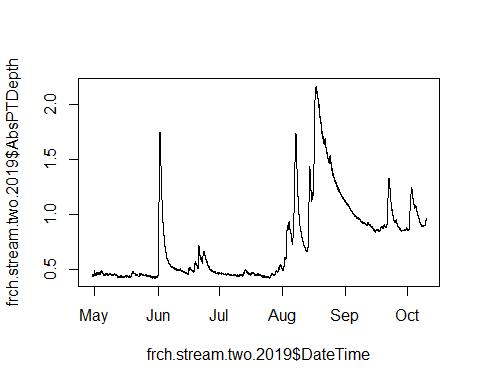
\includegraphics{Final_Q_files/figure-latex/unnamed-chunk-34-1.pdf}

This is the final discharge plot from the RC without the HOBO ware
points

\hypertarget{export-pt-data-to-csv-to-dod_discharge-prredicted_discharge-2018}{%
\subsubsection{export PT data to csv to
DoD\_Discharge-\textgreater Prredicted\_Discharge-\textgreater2018}\label{export-pt-data-to-csv-to-dod_discharge-prredicted_discharge-2018}}

\hypertarget{french-creek}{%
\subsection{French Creek}\label{french-creek}}

\hypertarget{raw-rating-curve-french-1-pressure-transducer}{%
\subsubsection{Raw Rating Curve French 1 Pressure
Transducer}\label{raw-rating-curve-french-1-pressure-transducer}}

\begin{verbatim}
## Joining, by = "DateTime"
\end{verbatim}

\begin{verbatim}
## `geom_smooth()` using formula 'y ~ x'
\end{verbatim}

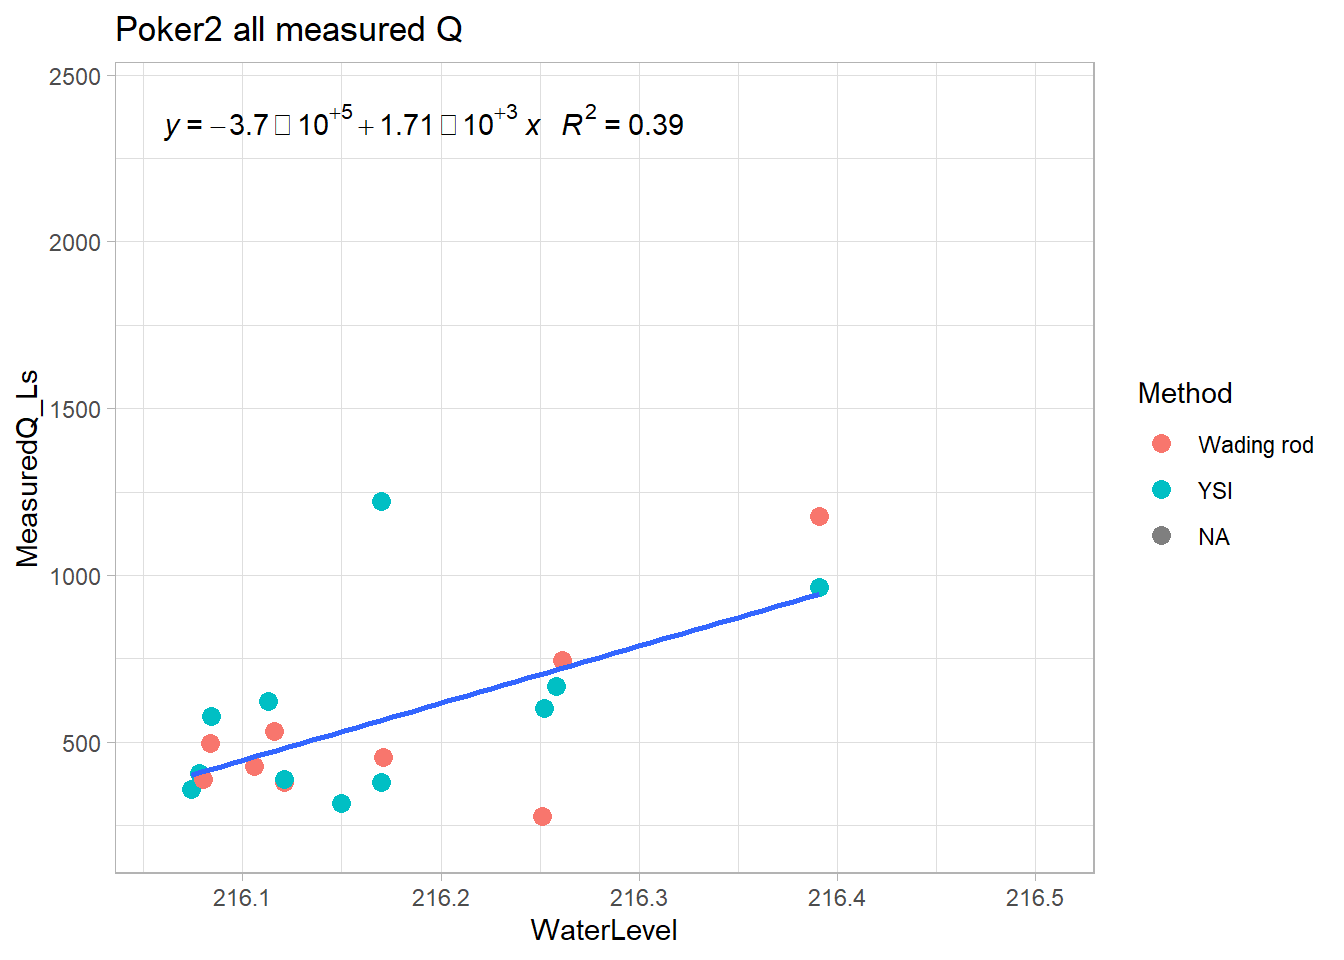
\includegraphics{Final_Q_files/figure-latex/unnamed-chunk-36-1.pdf}

\begin{verbatim}
## 
## Call:
## lm(formula = French1comb$MeasuredQ_Ls ~ French1comb$WaterLevelmeters)
## 
## Residuals:
##     Min      1Q  Median      3Q     Max 
## -195.36  -46.80  -11.97   41.21  176.95 
## 
## Coefficients:
##                               Estimate Std. Error t value Pr(>|t|)    
## (Intercept)                  -198904.1    38127.3  -5.217 0.000392 ***
## French1comb$WaterLevelmeters    1081.3      206.7   5.233 0.000383 ***
## ---
## Signif. codes:  0 '***' 0.001 '**' 0.01 '*' 0.05 '.' 0.1 ' ' 1
## 
## Residual standard error: 105.5 on 10 degrees of freedom
##   (6510 observations deleted due to missingness)
## Multiple R-squared:  0.7325, Adjusted R-squared:  0.7057 
## F-statistic: 27.38 on 1 and 10 DF,  p-value: 0.0003829
\end{verbatim}

Will remove the two HOBOware points

\begin{verbatim}
## Joining, by = "DateTime"
\end{verbatim}

\begin{verbatim}
## `geom_smooth()` using formula 'y ~ x'
\end{verbatim}

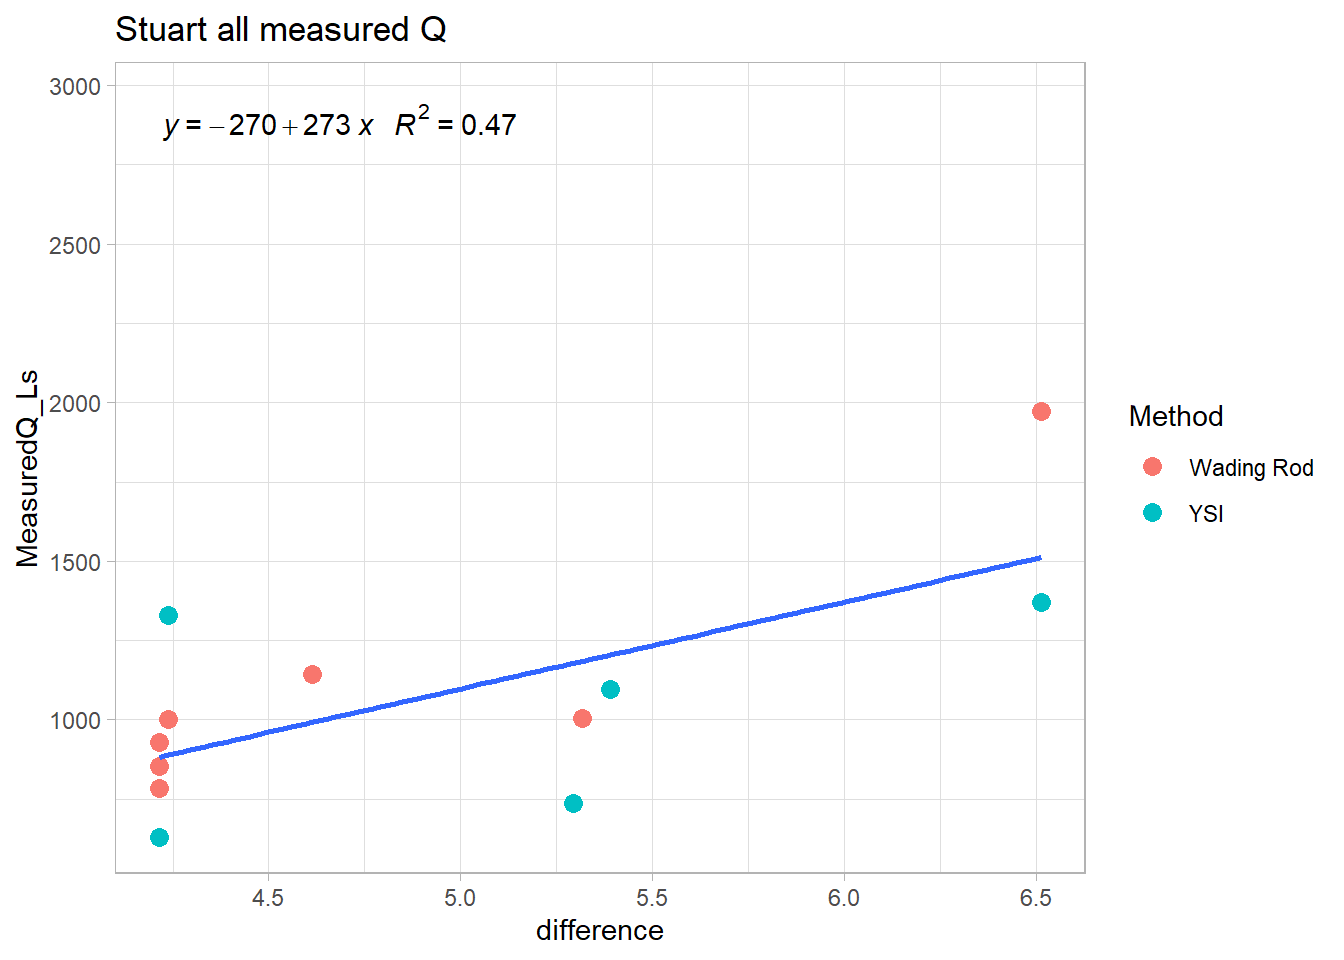
\includegraphics{Final_Q_files/figure-latex/unnamed-chunk-37-1.pdf}

\begin{verbatim}
## 
## Call:
## lm(formula = French1comb$MeasuredQ_Ls ~ French1comb$WaterLevelmeters)
## 
## Residuals:
##     Min      1Q  Median      3Q     Max 
## -195.36  -46.80  -11.97   41.21  176.95 
## 
## Coefficients:
##                               Estimate Std. Error t value Pr(>|t|)    
## (Intercept)                  -198904.1    38127.3  -5.217 0.000392 ***
## French1comb$WaterLevelmeters    1081.3      206.7   5.233 0.000383 ***
## ---
## Signif. codes:  0 '***' 0.001 '**' 0.01 '*' 0.05 '.' 0.1 ' ' 1
## 
## Residual standard error: 105.5 on 10 degrees of freedom
##   (6510 observations deleted due to missingness)
## Multiple R-squared:  0.7325, Adjusted R-squared:  0.7057 
## F-statistic: 27.38 on 1 and 10 DF,  p-value: 0.0003829
\end{verbatim}

\begin{enumerate}
\def\labelenumi{\arabic{enumi})}
\tightlist
\item
  Removed the HOBOware points
\end{enumerate}

\hypertarget{french-1-calculated-q-ls-1}{%
\subsection{French 1 Calculated Q
(L/s)}\label{french-1-calculated-q-ls-1}}

\hypertarget{black-points-are-observed-q-3}{%
\paragraph{Black points are observed
Q}\label{black-points-are-observed-q-3}}

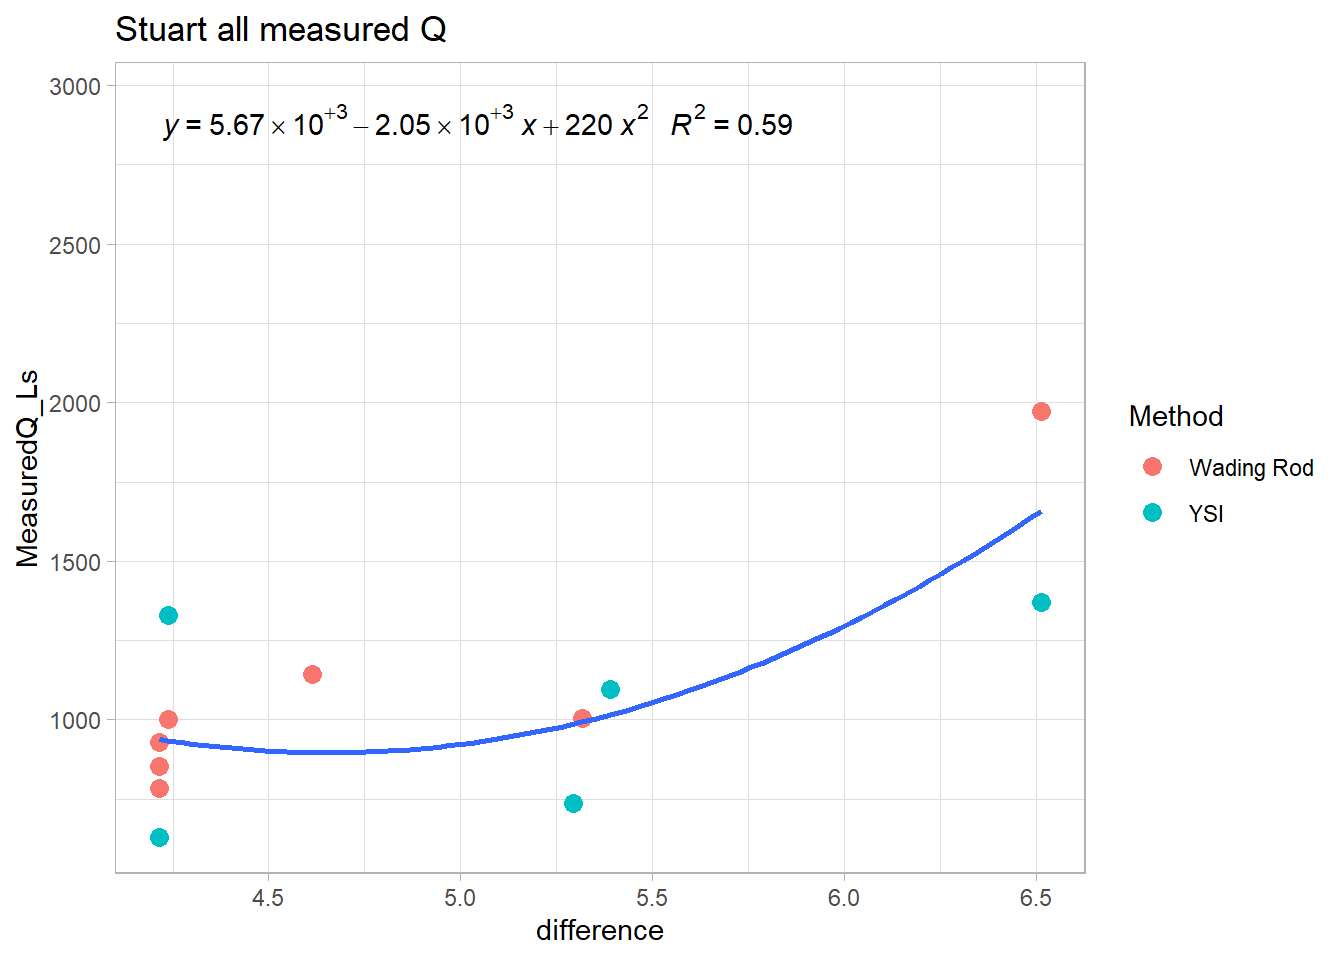
\includegraphics{Final_Q_files/figure-latex/unnamed-chunk-38-1.pdf} This
doesnt look too shabby!

\hypertarget{export-pt-data-to-csv-to-dod_discharge-prredicted_discharge-2018-1}{%
\subsubsection{export PT data to csv to
DoD\_Discharge-\textgreater Prredicted\_Discharge-\textgreater2018}\label{export-pt-data-to-csv-to-dod_discharge-prredicted_discharge-2018-1}}

\hypertarget{export-pt-data-to-csv-to-dod_discharge-prredicted_discharge-2018-2}{%
\subsubsection{export PT data to csv to
DoD\_Discharge-\textgreater Prredicted\_Discharge-\textgreater2018}\label{export-pt-data-to-csv-to-dod_discharge-prredicted_discharge-2018-2}}

\begin{itemize}
\tightlist
\item
  We rock at discharge!!!
\end{itemize}

2019 data is read from DoD-\textgreater2019 AK sensors-\textgreater2019
Sensor data -\textgreater PT-\textgreater DoD 2019 PT depth corrected
for atm\\
Wading rods and slugs were used to measure discrete Q during site visit
Includes all sites (Moose, French, Poker, Vault, Stuart)

\#2019 data is read in from DoD-\textgreater2019 ak
sensors-\textgreater2019 sensor data-\textgreater Q -\textgreater{}
Pressure Transducer Data-\textgreater Depth-\textgreater{}`site'

\hypertarget{checking-closeness-between-the-two-pressure-transducers-1}{%
\subparagraph{Checking closeness between the two Pressure
Transducers}\label{checking-closeness-between-the-two-pressure-transducers-1}}

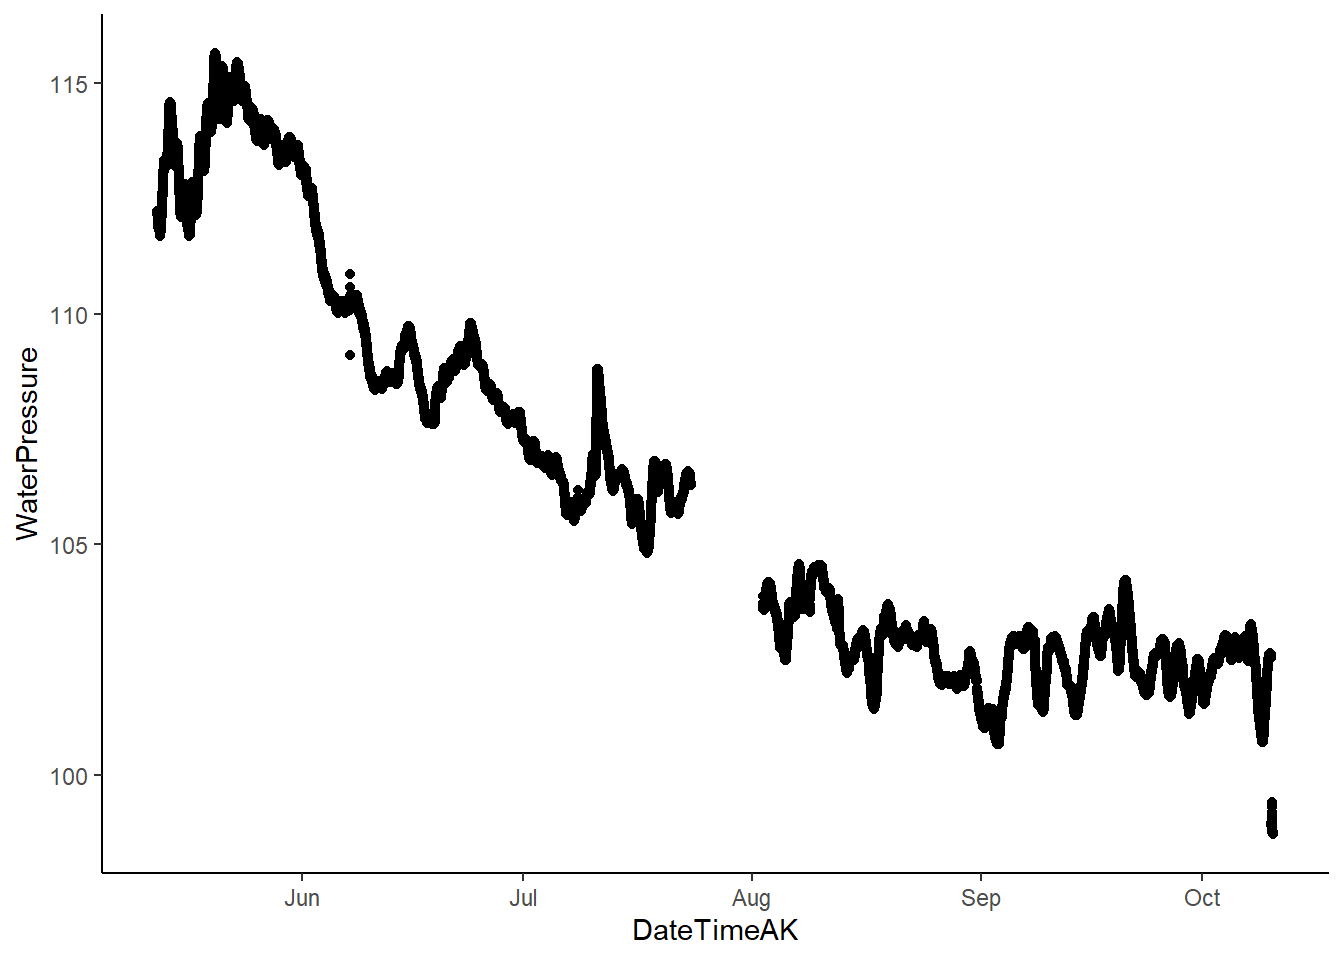
\includegraphics{Final_Q_files/figure-latex/unnamed-chunk-42-1.pdf}
Looks pretty good

\hypertarget{checking-raw-pt-data-1}{%
\subparagraph{Checking Raw PT data}\label{checking-raw-pt-data-1}}

\hypertarget{raw-moose-2}{%
\subsection{Raw Moose}\label{raw-moose-2}}

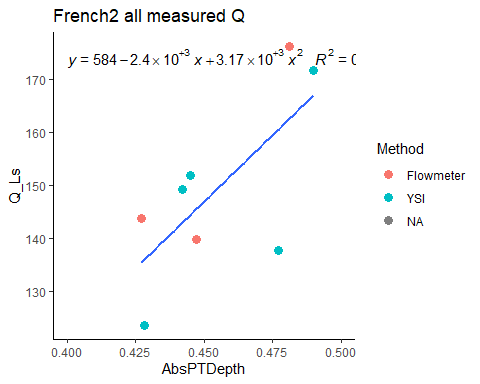
\includegraphics{Final_Q_files/figure-latex/unnamed-chunk-43-1.pdf} let
the cleaning commence! \#\# Moose 2.0 \#\#
\includegraphics{Final_Q_files/figure-latex/unnamed-chunk-44-1.pdf}
1)removed vertical bars in dataframe ? Spike in early Julyish does have
rainfall close to it\ldots.is it real? Middle of October? Ice on? Should
I clip middle of October, French was removed on October 10th according
to the field notebook

\hypertarget{export-pt-data-to-csv-to-dod_discharge-pt_data-2019}{%
\subsubsection{export PT data to csv to
DoD\_Discharge-\textgreater PT\_data-\textgreater2019}\label{export-pt-data-to-csv-to-dod_discharge-pt_data-2019}}

\hypertarget{observed-discharge-at-all-sites}{%
\subsubsection{Observed Discharge at all
sites}\label{observed-discharge-at-all-sites}}

Slugs and wading rods were used for 2019 observed Q

\includegraphics{Final_Q_files/figure-latex/unnamed-chunk-46-1.pdf}
\includegraphics{Final_Q_files/figure-latex/unnamed-chunk-46-2.pdf}
\includegraphics{Final_Q_files/figure-latex/unnamed-chunk-46-3.pdf}
\includegraphics{Final_Q_files/figure-latex/unnamed-chunk-46-4.pdf}
\includegraphics{Final_Q_files/figure-latex/unnamed-chunk-46-5.pdf}
\includegraphics{Final_Q_files/figure-latex/unnamed-chunk-46-6.pdf}
\includegraphics{Final_Q_files/figure-latex/unnamed-chunk-46-7.pdf}
\#\#\# Raw Rating Curve with Moose 1 Pressure Transducer

\begin{verbatim}
## Joining, by = c("Site", "DateTime")
\end{verbatim}

\begin{verbatim}
## 
## Call:
## lm(formula = Moose1comb.2019$Q_Ls ~ Moose1comb.2019$AbsPTDepth)
## 
## Residuals:
##     Min      1Q  Median      3Q     Max 
## -236.06 -127.32  -42.25    8.70  699.33 
## 
## Coefficients:
##                            Estimate Std. Error t value Pr(>|t|)    
## (Intercept)                 -1460.6      410.3  -3.560 0.006118 ** 
## Moose1comb.2019$AbsPTDepth   1969.8      332.5   5.925 0.000222 ***
## ---
## Signif. codes:  0 '***' 0.001 '**' 0.01 '*' 0.05 '.' 0.1 ' ' 1
## 
## Residual standard error: 268.2 on 9 degrees of freedom
##   (13789 observations deleted due to missingness)
## Multiple R-squared:  0.7959, Adjusted R-squared:  0.7733 
## F-statistic:  35.1 on 1 and 9 DF,  p-value: 0.0002221
\end{verbatim}

\begin{verbatim}
## `geom_smooth()` using formula 'y ~ x'
\end{verbatim}

\includegraphics{Final_Q_files/figure-latex/unnamed-chunk-47-1.pdf} Not
too shabby, im going to remove the top YSI point

\hypertarget{raw-rating-curve-with-moose-1-pressure-transducer-2}{%
\subsubsection{Raw Rating Curve with Moose 1 Pressure
Transducer}\label{raw-rating-curve-with-moose-1-pressure-transducer-2}}

\begin{verbatim}
## Joining, by = c("Site", "DateTime")
\end{verbatim}

\begin{verbatim}
## 
## Call:
## lm(formula = Moose2comb.2019$Q_Ls ~ Moose2comb.2019$AbsPTDepth)
## 
## Residuals:
##      Min       1Q   Median       3Q      Max 
## -175.338  -51.427   -5.621   46.981  218.936 
## 
## Coefficients:
##                            Estimate Std. Error t value Pr(>|t|)    
## (Intercept)                 -1384.5      171.3  -8.085 4.05e-05 ***
## Moose2comb.2019$AbsPTDepth   1848.0      139.7  13.231 1.02e-06 ***
## ---
## Signif. codes:  0 '***' 0.001 '**' 0.01 '*' 0.05 '.' 0.1 ' ' 1
## 
## Residual standard error: 111.7 on 8 degrees of freedom
##   (13790 observations deleted due to missingness)
## Multiple R-squared:  0.9563, Adjusted R-squared:  0.9508 
## F-statistic: 175.1 on 1 and 8 DF,  p-value: 1.015e-06
\end{verbatim}

\begin{verbatim}
## `geom_smooth()` using formula 'y ~ x'
\end{verbatim}

\includegraphics{Final_Q_files/figure-latex/unnamed-chunk-48-1.pdf}
That's better, I will use this for the predicted discharge

\hypertarget{predicted-q-moos-pt1}{%
\subsubsection{Predicted Q MOOS PT1}\label{predicted-q-moos-pt1}}

\hypertarget{black-points-are-observed-q-4}{%
\paragraph{Black points are observed
Q}\label{black-points-are-observed-q-4}}

\includegraphics{Final_Q_files/figure-latex/unnamed-chunk-49-1.pdf} Not
too shabby

\hypertarget{export-pt-data-to-csv-to-dod_discharge-predicted_discharge-2019}{%
\subsubsection{export PT data to csv to
DoD\_Discharge-\textgreater Predicted\_discharge-\textgreater2019}\label{export-pt-data-to-csv-to-dod_discharge-predicted_discharge-2019}}

\hypertarget{raw-french-pt1}{%
\subsection{Raw French PT1}\label{raw-french-pt1}}

\includegraphics{Final_Q_files/figure-latex/unnamed-chunk-51-1.pdf}
Looks good. I am going to replace the noisy-ness of the receding limb in
the big august storm with FRCH PT2 as it is less noisy let the cleaning
commence!

\hypertarget{frch-pt1-2.0}{%
\section{FRCH PT1 2.0}\label{frch-pt1-2.0}}

\begin{verbatim}
## [1] 10549
\end{verbatim}

\includegraphics{Final_Q_files/figure-latex/unnamed-chunk-52-1.pdf}
\includegraphics{Final_Q_files/figure-latex/unnamed-chunk-52-2.pdf} 1)
replaced the noisy receding limb in the big end of August storm of PT1
with the more constant data of PT2

\hypertarget{raw-french-pt2}{%
\subsection{Raw French PT2}\label{raw-french-pt2}}

\includegraphics{Final_Q_files/figure-latex/unnamed-chunk-53-1.pdf}
Going to clean some of the vertical bars in may but other than that this
looks pretty good! let the cleaning commence \#\# FRCH PT2 2.0
\includegraphics{Final_Q_files/figure-latex/unnamed-chunk-54-1.pdf} 1)
removed vertical bars early on in season

\hypertarget{export-pt-data-to-csv-to-dod_discharge-pt_data-2019-1}{%
\subsubsection{export PT data to csv to
DoD\_Discharge-\textgreater PT\_data-\textgreater2019}\label{export-pt-data-to-csv-to-dod_discharge-pt_data-2019-1}}

\hypertarget{raw-rating-curve-with-french-1-pressure-transducer-1}{%
\subsubsection{Raw Rating Curve with French 1 Pressure
Transducer}\label{raw-rating-curve-with-french-1-pressure-transducer-1}}

\begin{verbatim}
## Joining, by = c("Site", "DateTime")
\end{verbatim}

\begin{verbatim}
## 
## Call:
## lm(formula = French1comb.2019$Q_Ls ~ French1comb.2019$AbsPTDepth)
## 
## Residuals:
##     Min      1Q  Median      3Q     Max 
## -371.71  -46.80  -13.33   25.72  749.71 
## 
## Coefficients:
##                             Estimate Std. Error t value Pr(>|t|)    
## (Intercept)                  -1015.5      259.5  -3.914 0.002893 ** 
## French1comb.2019$AbsPTDepth   1860.6      320.8   5.800 0.000173 ***
## ---
## Signif. codes:  0 '***' 0.001 '**' 0.01 '*' 0.05 '.' 0.1 ' ' 1
## 
## Residual standard error: 285.8 on 10 degrees of freedom
##   (15711 observations deleted due to missingness)
## Multiple R-squared:  0.7709, Adjusted R-squared:  0.748 
## F-statistic: 33.64 on 1 and 10 DF,  p-value: 0.0001729
\end{verbatim}

\begin{verbatim}
## `geom_smooth()` using formula 'y ~ x'
\end{verbatim}

\includegraphics{Final_Q_files/figure-latex/unnamed-chunk-56-1.pdf} Lots
of points that are clustered at the bottom. I will remove the 3 large
YSI points

\begin{verbatim}
## Joining, by = c("Site", "DateTime")
\end{verbatim}

\begin{verbatim}
## 
## Call:
## lm(formula = French2comb.2019$Q_Ls ~ French2comb.2019$AbsPTDepth)
## 
## Residuals:
##     Min      1Q  Median      3Q     Max 
## -36.779  -7.224   3.299  13.574  18.547 
## 
## Coefficients:
##                             Estimate Std. Error t value Pr(>|t|)
## (Intercept)                   -173.4      192.8  -0.899    0.398
## French2comb.2019$AbsPTDepth    507.9      307.4   1.652    0.142
## 
## Residual standard error: 19.08 on 7 degrees of freedom
##   (15714 observations deleted due to missingness)
## Multiple R-squared:  0.2805, Adjusted R-squared:  0.1778 
## F-statistic:  2.73 on 1 and 7 DF,  p-value: 0.1425
\end{verbatim}

\begin{verbatim}
## `geom_smooth()` using formula 'y ~ x'
\end{verbatim}

\includegraphics{Final_Q_files/figure-latex/unnamed-chunk-57-1.pdf} Not
as good of an R\^{}2

\hypertarget{raw-rating-curve-with-french-2-pressure-transducer}{%
\subsubsection{Raw Rating Curve with French 2 Pressure
Transducer}\label{raw-rating-curve-with-french-2-pressure-transducer}}

\begin{verbatim}
## Joining, by = c("Site", "DateTime")
\end{verbatim}

\begin{verbatim}
## 
## Call:
## lm(formula = French3comb.2019$Q_Ls ~ French3comb.2019$AbsPTDepth)
## 
## Residuals:
##     Min      1Q  Median      3Q     Max 
## -358.33  -44.52   -5.42   24.09  732.91 
## 
## Coefficients:
##                             Estimate Std. Error t value Pr(>|t|)    
## (Intercept)                   -658.4      199.2  -3.306 0.007936 ** 
## French3comb.2019$AbsPTDepth   1771.3      300.9   5.887 0.000154 ***
## ---
## Signif. codes:  0 '***' 0.001 '**' 0.01 '*' 0.05 '.' 0.1 ' ' 1
## 
## Residual standard error: 282.6 on 10 degrees of freedom
##   (15708 observations deleted due to missingness)
## Multiple R-squared:  0.7761, Adjusted R-squared:  0.7537 
## F-statistic: 34.65 on 1 and 10 DF,  p-value: 0.0001538
\end{verbatim}

\begin{verbatim}
## `geom_smooth()` using formula 'y ~ x'
\end{verbatim}

\includegraphics{Final_Q_files/figure-latex/unnamed-chunk-58-1.pdf} Same
thing as FRCH 1. Next plot will be without the 3 high YSI points

\begin{verbatim}
## Joining, by = c("Site", "DateTime")
\end{verbatim}

\begin{verbatim}
## 
## Call:
## lm(formula = French2comb.2019$Q_Ls ~ French2comb.2019$AbsPTDepth)
## 
## Residuals:
##     Min      1Q  Median      3Q     Max 
## -36.779  -7.224   3.299  13.574  18.547 
## 
## Coefficients:
##                             Estimate Std. Error t value Pr(>|t|)
## (Intercept)                   -173.4      192.8  -0.899    0.398
## French2comb.2019$AbsPTDepth    507.9      307.4   1.652    0.142
## 
## Residual standard error: 19.08 on 7 degrees of freedom
##   (15714 observations deleted due to missingness)
## Multiple R-squared:  0.2805, Adjusted R-squared:  0.1778 
## F-statistic:  2.73 on 1 and 7 DF,  p-value: 0.1425
\end{verbatim}

\begin{verbatim}
## `geom_smooth()` using formula 'y ~ x'
\end{verbatim}

\includegraphics{Final_Q_files/figure-latex/unnamed-chunk-59-1.pdf} I
will remove the low flowmeter point for the next plot

\begin{verbatim}
## Joining, by = c("Site", "DateTime")
\end{verbatim}

\begin{verbatim}
## 
## Call:
## lm(formula = French5comb.2019$Q_Ls ~ French5comb.2019$AbsPTDepth)
## 
## Residuals:
##     Min      1Q  Median      3Q     Max 
## -360.35  -48.27    1.21   18.96  732.37 
## 
## Coefficients:
##                             Estimate Std. Error t value Pr(>|t|)    
## (Intercept)                   -649.5      217.5  -2.987 0.015275 *  
## French5comb.2019$AbsPTDepth   1763.4      321.0   5.493 0.000384 ***
## ---
## Signif. codes:  0 '***' 0.001 '**' 0.01 '*' 0.05 '.' 0.1 ' ' 1
## 
## Residual standard error: 297.5 on 9 degrees of freedom
##   (15709 observations deleted due to missingness)
## Multiple R-squared:  0.7703, Adjusted R-squared:  0.7447 
## F-statistic: 30.17 on 1 and 9 DF,  p-value: 0.0003836
\end{verbatim}

\begin{verbatim}
## `geom_smooth()` using formula 'y ~ x'
\end{verbatim}

\includegraphics{Final_Q_files/figure-latex/unnamed-chunk-60-1.pdf} This
is the RC I will use for predicted Q

\hypertarget{predicted-q-frch-pt1}{%
\subsubsection{Predicted Q FRCH PT1}\label{predicted-q-frch-pt1}}

\hypertarget{black-points-are-observed-q-5}{%
\paragraph{Black points are observed
Q}\label{black-points-are-observed-q-5}}

\includegraphics{Final_Q_files/figure-latex/unnamed-chunk-61-1.pdf}
Without a big range in observed Q this is the best we can do

\hypertarget{predicted-q-frch-pt2}{%
\subsubsection{Predicted Q FRCH PT2}\label{predicted-q-frch-pt2}}

\hypertarget{black-points-are-observed-q-6}{%
\paragraph{Black points are observed
Q}\label{black-points-are-observed-q-6}}

\includegraphics{Final_Q_files/figure-latex/unnamed-chunk-62-1.pdf} This
gives us much higher Q

\hypertarget{compare-frch-pt1-and-pt2}{%
\subsubsection{Compare FRCH PT1 and
PT2}\label{compare-frch-pt1-and-pt2}}

\includegraphics{Final_Q_files/figure-latex/unnamed-chunk-63-1.pdf} When
it comes to the higher Q they are way off.

\hypertarget{export-pt-data-to-csv-to-dod_discharge-predicted_discharge-2019-1}{%
\subsubsection{export PT data to csv to
DoD\_Discharge-\textgreater Predicted\_Discharge-\textgreater2019}\label{export-pt-data-to-csv-to-dod_discharge-predicted_discharge-2019-1}}

\hypertarget{raw-poker-pt1}{%
\subsection{Raw Poker PT1}\label{raw-poker-pt1}}

\includegraphics{Final_Q_files/figure-latex/unnamed-chunk-65-1.pdf} THe
beginning increase appears to be real with the precip on top. I need to
remove some of the "vertical bars within the data frame and check take
out date. I am also going to take out the beaver dam tha is there from
late august to middle of september Let the cleaning commence!

\includegraphics{Final_Q_files/figure-latex/unnamed-chunk-66-1.pdf} 1)
Removed vertical bars early on in dataset 2) Removed beaver dam related
data entirely 3) removed end of season out of water points

\hypertarget{raw-poker-pt2}{%
\subsection{Raw Poker PT2}\label{raw-poker-pt2}}

\includegraphics{Final_Q_files/figure-latex/unnamed-chunk-67-1.pdf} Same
procedure as PT1\ldots.let the cleaning commence!

\includegraphics{Final_Q_files/figure-latex/unnamed-chunk-68-1.pdf} 1)
Removed vertical bars early on in dataset 2) Removed beaver dam related
data entirely 3) removed end of season out of water points

\hypertarget{export-pt-data-to-csv-to-dod_discharge-pt_data-2019-2}{%
\subsubsection{export PT data to csv to
DoD\_Discharge-\textgreater PT\_data-\textgreater2019}\label{export-pt-data-to-csv-to-dod_discharge-pt_data-2019-2}}

\hypertarget{raw-rating-curve-with-poker-1-pressure-transducer}{%
\subsubsection{Raw Rating Curve with Poker 1 Pressure
Transducer}\label{raw-rating-curve-with-poker-1-pressure-transducer}}

\begin{verbatim}
## Joining, by = c("Site", "DateTime")
\end{verbatim}

\begin{verbatim}
## 
## Call:
## lm(formula = Poker1comb.2019$Q_Ls ~ Poker1comb.2019$AbsPTDepth)
## 
## Residuals:
##     Min      1Q  Median      3Q     Max 
## -169.60  -59.12  -12.96   30.48  208.98 
## 
## Coefficients:
##                            Estimate Std. Error t value Pr(>|t|)   
## (Intercept)                  198.93      56.85   3.499  0.00809 **
## Poker1comb.2019$AbsPTDepth   787.07     242.75   3.242  0.01184 * 
## ---
## Signif. codes:  0 '***' 0.001 '**' 0.01 '*' 0.05 '.' 0.1 ' ' 1
## 
## Residual standard error: 111.2 on 8 degrees of freedom
##   (13799 observations deleted due to missingness)
## Multiple R-squared:  0.5679, Adjusted R-squared:  0.5138 
## F-statistic: 10.51 on 1 and 8 DF,  p-value: 0.01184
\end{verbatim}

\begin{verbatim}
## `geom_smooth()` using formula 'y ~ x'
\end{verbatim}

\includegraphics{Final_Q_files/figure-latex/unnamed-chunk-70-1.pdf} I
will remove the highest flowmeter point

\begin{verbatim}
## Joining, by = c("Site", "DateTime")
\end{verbatim}

\begin{verbatim}
## 
## Call:
## lm(formula = Poker2comb.2019$Q_Ls ~ Poker2comb.2019$AbsPTDepth)
## 
## Residuals:
##     Min      1Q  Median      3Q     Max 
## -98.837 -55.986  -1.269  37.849 130.892 
## 
## Coefficients:
##                            Estimate Std. Error t value Pr(>|t|)    
## (Intercept)                  222.06      37.73   5.886 0.000608 ***
## Poker2comb.2019$AbsPTDepth   499.94     179.26   2.789 0.026949 *  
## ---
## Signif. codes:  0 '***' 0.001 '**' 0.01 '*' 0.05 '.' 0.1 ' ' 1
## 
## Residual standard error: 72.63 on 7 degrees of freedom
##   (13800 observations deleted due to missingness)
## Multiple R-squared:  0.5263, Adjusted R-squared:  0.4587 
## F-statistic: 7.778 on 1 and 7 DF,  p-value: 0.02695
\end{verbatim}

\begin{verbatim}
## `geom_smooth()` using formula 'y ~ x'
\end{verbatim}

\includegraphics{Final_Q_files/figure-latex/unnamed-chunk-71-1.pdf}
Worse R\^{}2, Ill use the raw one

\hypertarget{predicted-q-poke-pt1}{%
\subsubsection{Predicted Q POKE PT1}\label{predicted-q-poke-pt1}}

\hypertarget{black-points-are-observed-q-7}{%
\paragraph{Black points are observed
Q}\label{black-points-are-observed-q-7}}

\includegraphics{Final_Q_files/figure-latex/unnamed-chunk-72-1.pdf}

Not the worst thing I've seen in the world

\hypertarget{raw-rating-curve-with-poker-2-pressure-transducer}{%
\subsubsection{Raw Rating Curve with Poker 2 Pressure
Transducer}\label{raw-rating-curve-with-poker-2-pressure-transducer}}

\begin{verbatim}
## Joining, by = c("Site", "DateTime")
\end{verbatim}

\begin{verbatim}
## 
## Call:
## lm(formula = Poker2comb.2019$Q_Ls ~ Poker2comb.2019$AbsPTDepth)
## 
## Residuals:
##     Min      1Q  Median      3Q     Max 
## -128.21  -78.42   28.37   31.08  168.99 
## 
## Coefficients:
##                            Estimate Std. Error t value Pr(>|t|)   
## (Intercept)                  -285.8      160.2  -1.784  0.11759   
## Poker2comb.2019$AbsPTDepth   1648.8      410.9   4.012  0.00511 **
## ---
## Signif. codes:  0 '***' 0.001 '**' 0.01 '*' 0.05 '.' 0.1 ' ' 1
## 
## Residual standard error: 99.57 on 7 degrees of freedom
##   (13517 observations deleted due to missingness)
## Multiple R-squared:  0.697,  Adjusted R-squared:  0.6537 
## F-statistic:  16.1 on 1 and 7 DF,  p-value: 0.005109
\end{verbatim}

\begin{verbatim}
## `geom_smooth()` using formula 'y ~ x'
\end{verbatim}

\includegraphics{Final_Q_files/figure-latex/unnamed-chunk-73-1.pdf}
\#\#\# Predicted Q POKE PT2 \#\#\#\# Black points are observed Q

\includegraphics{Final_Q_files/figure-latex/unnamed-chunk-74-1.pdf}

\hypertarget{average-poke-q}{%
\subsubsection{Average POKE Q}\label{average-poke-q}}

\includegraphics{Final_Q_files/figure-latex/unnamed-chunk-75-1.pdf}

\hypertarget{export-pt-data-to-csv-to-dod_discharge-predicted_discharge-2019-2}{%
\subsubsection{export PT data to csv to
DoD\_Discharge-\textgreater Predicted\_Discharge-\textgreater2019}\label{export-pt-data-to-csv-to-dod_discharge-predicted_discharge-2019-2}}

\hypertarget{raw-vault-pt1}{%
\subsection{Raw Vault PT1}\label{raw-vault-pt1}}

\includegraphics{Final_Q_files/figure-latex/unnamed-chunk-77-1.pdf} Out
of water at the end of the year? Let the cleaning commence!

\includegraphics{Final_Q_files/figure-latex/unnamed-chunk-78-1.pdf} 1)
Removed end of record as there were erroneous points that might have
been from ice on and then also out of water points

\hypertarget{export-pt-data-to-csv-to-dod_discharge-pt_data-2019-3}{%
\subsubsection{export PT data to csv to
DoD\_Discharge-\textgreater PT\_data-\textgreater2019}\label{export-pt-data-to-csv-to-dod_discharge-pt_data-2019-3}}

\hypertarget{raw-rating-curve-with-vaul-pt1}{%
\subsubsection{Raw Rating Curve with VAUL
PT1}\label{raw-rating-curve-with-vaul-pt1}}

\begin{verbatim}
## Joining, by = c("Site", "DateTime")
\end{verbatim}

\begin{verbatim}
## 
## Call:
## lm(formula = Vaultcomb.2019$Q_Ls ~ 0 + Vaultcomb.2019$AbsPTDepth)
## 
## Residuals:
##    Min     1Q Median     3Q    Max 
## -86.91 -76.88 -41.14  54.53 169.09 
## 
## Coefficients:
##                           Estimate Std. Error t value Pr(>|t|)   
## Vaultcomb.2019$AbsPTDepth   200.67      58.77   3.415  0.00769 **
## ---
## Signif. codes:  0 '***' 0.001 '**' 0.01 '*' 0.05 '.' 0.1 ' ' 1
## 
## Residual standard error: 94.22 on 9 degrees of freedom
##   (12731 observations deleted due to missingness)
## Multiple R-squared:  0.5644, Adjusted R-squared:  0.516 
## F-statistic: 11.66 on 1 and 9 DF,  p-value: 0.007692
\end{verbatim}

\begin{verbatim}
## `geom_smooth()` using formula 'y ~ x'
\end{verbatim}

\includegraphics{Final_Q_files/figure-latex/unnamed-chunk-80-1.pdf}
Maybe I can take the high points about the line but i am going to keep
it for right now

\#\#\# Predicted Q VAULPT1 \#\#\#\# Black points are observed Q

\includegraphics{Final_Q_files/figure-latex/unnamed-chunk-81-1.pdf} Not
great\ldots..

\hypertarget{export-pt-data-to-csv-to-dod_discharge-predicted_discharge-2019-3}{%
\subsubsection{export PT data to csv to
DoD\_Discharge-\textgreater Predicted\_Discharge-\textgreater2019}\label{export-pt-data-to-csv-to-dod_discharge-predicted_discharge-2019-3}}

\hypertarget{raw-stuart-pt1}{%
\subsection{Raw Stuart PT1}\label{raw-stuart-pt1}}

\includegraphics{Final_Q_files/figure-latex/unnamed-chunk-83-1.pdf}
Stuart PT1 only has record until 8/23\ldots{} Looks pretty clean though

\hypertarget{raw-stuart-pt2}{%
\subsection{Raw Stuart PT2}\label{raw-stuart-pt2}}

\includegraphics{Final_Q_files/figure-latex/unnamed-chunk-84-1.pdf} Just
looks like I need to clip out the end of the season points
there\ldots Let the cleaning commence!

\hypertarget{strt-pt2-2.0}{%
\subsubsection{STRT PT2 2.0}\label{strt-pt2-2.0}}

\includegraphics{Final_Q_files/figure-latex/unnamed-chunk-85-1.pdf} 1)
removed out of water points at the end of the season

\hypertarget{export-pt-data-to-csv-to-dod_discharge-pt_data-2019-4}{%
\subsubsection{export PT data to csv to
DoD\_Discharge-\textgreater PT\_data-\textgreater2019}\label{export-pt-data-to-csv-to-dod_discharge-pt_data-2019-4}}

\hypertarget{raw-rating-curve-with-strt-pt1}{%
\subsubsection{Raw Rating Curve with STRT
PT1}\label{raw-rating-curve-with-strt-pt1}}

\begin{verbatim}
## Joining, by = c("Site", "DateTime")
\end{verbatim}

\begin{verbatim}
## 
## Call:
## lm(formula = Stuart1comb.2019$Q_Ls ~ Stuart1comb.2019$AbsPTDepth)
## 
## Residuals:
##    1426    1428    2776    3447    3452    7478    8246 
## -632.66 -181.02   85.74 -141.83  810.31 -117.82  177.28 
## 
## Coefficients:
##                             Estimate Std. Error t value Pr(>|t|)    
## (Intercept)                   -732.6      339.8  -2.156 0.083610 .  
## Stuart1comb.2019$AbsPTDepth   3823.0      446.1   8.570 0.000356 ***
## ---
## Signif. codes:  0 '***' 0.001 '**' 0.01 '*' 0.05 '.' 0.1 ' ' 1
## 
## Residual standard error: 482.2 on 5 degrees of freedom
##   (9018 observations deleted due to missingness)
## Multiple R-squared:  0.9363, Adjusted R-squared:  0.9235 
## F-statistic: 73.45 on 1 and 5 DF,  p-value: 0.0003564
\end{verbatim}

\begin{verbatim}
## `geom_smooth()` using formula 'y ~ x'
\end{verbatim}

\includegraphics{Final_Q_files/figure-latex/unnamed-chunk-87-1.pdf} I
think the first time I did this RC we ook out the two large Flowmeter
calculations but then that gives us a negative relationship which makes
the predicted Q really bad

\hypertarget{raw-rating-curve-with-strt-pt2}{%
\subsubsection{Raw Rating Curve with STRT
PT2}\label{raw-rating-curve-with-strt-pt2}}

\begin{verbatim}
## Joining, by = c("Site", "DateTime")
\end{verbatim}

\begin{verbatim}
## 
## Call:
## lm(formula = Stuart2comb.2019$Q_Ls ~ Stuart2comb.2019$AbsPTDepth)
## 
## Residuals:
##     Min      1Q  Median      3Q     Max 
## -1901.7 -1326.8  -797.3   168.5  4578.9 
## 
## Coefficients:
##                             Estimate Std. Error t value Pr(>|t|)  
## (Intercept)                   -54.74    1419.13  -0.039   0.9703  
## Stuart2comb.2019$AbsPTDepth  4905.18    1993.72   2.460   0.0434 *
## ---
## Signif. codes:  0 '***' 0.001 '**' 0.01 '*' 0.05 '.' 0.1 ' ' 1
## 
## Residual standard error: 2249 on 7 degrees of freedom
##   (13854 observations deleted due to missingness)
## Multiple R-squared:  0.4637, Adjusted R-squared:  0.3871 
## F-statistic: 6.053 on 1 and 7 DF,  p-value: 0.04345
\end{verbatim}

\begin{verbatim}
## `geom_smooth()` using formula 'y ~ x'
\end{verbatim}

\includegraphics{Final_Q_files/figure-latex/unnamed-chunk-88-1.pdf} I am
going to remove the high YSI pointt

\hypertarget{rating-curve-with-strt-pt2-2.0}{%
\subsubsection{Rating Curve with STRT PT2
2.0}\label{rating-curve-with-strt-pt2-2.0}}

\begin{verbatim}
## Joining, by = c("Site", "DateTime")
\end{verbatim}

\begin{verbatim}
## 
## Call:
## lm(formula = Stuart3comb.2019$Q_Ls ~ Stuart3comb.2019$AbsPTDepth)
## 
## Residuals:
##     Min      1Q  Median      3Q     Max 
## -946.69 -581.71 -458.34  -50.03 2922.95 
## 
## Coefficients:
##                             Estimate Std. Error t value Pr(>|t|)  
## (Intercept)                   -176.8      858.4  -0.206    0.844  
## Stuart3comb.2019$AbsPTDepth   4130.2     1223.8   3.375    0.015 *
## ---
## Signif. codes:  0 '***' 0.001 '**' 0.01 '*' 0.05 '.' 0.1 ' ' 1
## 
## Residual standard error: 1360 on 6 degrees of freedom
##   (13855 observations deleted due to missingness)
## Multiple R-squared:  0.655,  Adjusted R-squared:  0.5975 
## F-statistic: 11.39 on 1 and 6 DF,  p-value: 0.01495
\end{verbatim}

\begin{verbatim}
## `geom_smooth()` using formula 'y ~ x'
\end{verbatim}

\includegraphics{Final_Q_files/figure-latex/unnamed-chunk-89-1.pdf} Ill
remove the high flowmeter

\hypertarget{rating-curve-with-strt-pt2-2.0-1}{%
\subsubsection{Rating Curve with STRT PT2
2.0}\label{rating-curve-with-strt-pt2-2.0-1}}

\begin{verbatim}
## Joining, by = c("Site", "DateTime")
\end{verbatim}

\begin{verbatim}
## 
## Call:
## lm(formula = Stuart4comb.2019$Q_Ls ~ Stuart4comb.2019$AbsPTDepth)
## 
## Residuals:
##   1426   1428   2776   3447   3452   7478   8246 
## -615.3 -171.7   85.3 -159.5  804.0 -152.3  209.5 
## 
## Coefficients:
##                             Estimate Std. Error t value Pr(>|t|)    
## (Intercept)                   -382.6      305.0  -1.255  0.26509    
## Stuart4comb.2019$AbsPTDepth   3753.2      436.3   8.603  0.00035 ***
## ---
## Signif. codes:  0 '***' 0.001 '**' 0.01 '*' 0.05 '.' 0.1 ' ' 1
## 
## Residual standard error: 480.5 on 5 degrees of freedom
##   (13856 observations deleted due to missingness)
## Multiple R-squared:  0.9367, Adjusted R-squared:  0.9241 
## F-statistic: 74.01 on 1 and 5 DF,  p-value: 0.0003501
\end{verbatim}

\begin{verbatim}
## `geom_smooth()` using formula 'y ~ x'
\end{verbatim}

\includegraphics{Final_Q_files/figure-latex/unnamed-chunk-90-1.pdf}
1)Removed top flowmeter and YSI point

\hypertarget{predicted-q-strt-pt1}{%
\subsubsection{Predicted Q STRT PT1}\label{predicted-q-strt-pt1}}

\hypertarget{black-points-are-observed-q-8}{%
\paragraph{Black points are observed
Q}\label{black-points-are-observed-q-8}}

\includegraphics{Final_Q_files/figure-latex/unnamed-chunk-91-1.pdf}

\hypertarget{predicted-q-strt-pt2}{%
\subsubsection{Predicted Q STRT PT2}\label{predicted-q-strt-pt2}}

\hypertarget{black-points-are-observed-q-9}{%
\paragraph{Black points are observed
Q}\label{black-points-are-observed-q-9}}

\includegraphics{Final_Q_files/figure-latex/unnamed-chunk-92-1.pdf}

\hypertarget{average-strt-q}{%
\subsubsection{Average STRT Q}\label{average-strt-q}}

\includegraphics{Final_Q_files/figure-latex/unnamed-chunk-93-1.pdf}

\hypertarget{export-pt-data-to-csv-to-dod_discharge-predicted_discharge-2019-4}{%
\subsubsection{export PT data to csv to
DoD\_Discharge-\textgreater Predicted\_Discharge-\textgreater2019}\label{export-pt-data-to-csv-to-dod_discharge-predicted_discharge-2019-4}}

\hypertarget{export-pt-data-to-csv-to-dod_discharge-predicted_discharge-2019-5}{%
\subsubsection{export PT data to csv to
DoD\_Discharge-\textgreater Predicted\_Discharge-\textgreater2019}\label{export-pt-data-to-csv-to-dod_discharge-predicted_discharge-2019-5}}

2020 (Moose, French, Poker, Vault, Stuart), and 2021 (Moose, French,
Poker, Vault, Stuart), clean out of water points, potentially erroneous
points collected, beaver dams, etc. and prepare to convert to continuous
predicted discharge (Q) throuhgout the year.

2020 data is read in from DoD Project-\textgreater2020 AK
sensors-\textgreater Discharge-\textgreater Pressure
Transducer-\textgreater Water Level-\textgreater{}``site''

\hypertarget{comparing-pts}{%
\subsubsection{comparing PTs}\label{comparing-pts}}

\includegraphics{Final_Q_files/figure-latex/unnamed-chunk-97-1.pdf} Some
erroneous points but not bad. a slight shift

\hypertarget{comparing-frch}{%
\subsubsection{comparing FRCH}\label{comparing-frch}}

\includegraphics{Final_Q_files/figure-latex/unnamed-chunk-98-1.pdf}
Pretty good, have to clean some of those points

\hypertarget{comparing-frch-1}{%
\subsubsection{comparing FRCH}\label{comparing-frch-1}}

\includegraphics{Final_Q_files/figure-latex/unnamed-chunk-99-1.pdf}

Same as French, some erroneous points that will need to be cleaned

\includegraphics{Final_Q_files/figure-latex/unnamed-chunk-100-1.pdf} One
PT is definitely more noisy

\hypertarget{observed-discharge-at-all-sites-for-2020}{%
\subsubsection{Observed Discharge at all sites for
2020}\label{observed-discharge-at-all-sites-for-2020}}

Slugs and wading rods were used for 2020 observed Q

\includegraphics{Final_Q_files/figure-latex/unnamed-chunk-101-1.pdf}
\includegraphics{Final_Q_files/figure-latex/unnamed-chunk-101-2.pdf}
\includegraphics{Final_Q_files/figure-latex/unnamed-chunk-101-3.pdf}
\includegraphics{Final_Q_files/figure-latex/unnamed-chunk-101-4.pdf}
\includegraphics{Final_Q_files/figure-latex/unnamed-chunk-101-5.pdf}
\includegraphics{Final_Q_files/figure-latex/unnamed-chunk-101-6.pdf}
\includegraphics{Final_Q_files/figure-latex/unnamed-chunk-101-7.pdf}

\hypertarget{raw-moose-pt1}{%
\subsection{Raw Moose PT1}\label{raw-moose-pt1}}

\includegraphics{Final_Q_files/figure-latex/unnamed-chunk-102-1.pdf}
Noisy on the falling limb of first storm, potentially some out of water
points in August and at the end of the season\ldots Let the cleaning
commence!

\includegraphics{Final_Q_files/figure-latex/unnamed-chunk-103-1.pdf}

\begin{verbatim}
## [1] 166.093
\end{verbatim}

\begin{verbatim}
## [1] 165.977
\end{verbatim}

\begin{verbatim}
## [1] 0.116
\end{verbatim}

\begin{verbatim}
## Joining, by = c("Site", "DateTimeGMT", "AbsolutePressure", "WaterLevel", "DateTime")
\end{verbatim}

\includegraphics{Final_Q_files/figure-latex/unnamed-chunk-103-2.pdf} 1)
Clipped off data after 10/14 because thats when we took the PTs out 2)
Set receding limb of first big storm in June to NA due to ``noisy-ness''
3) clipped off errant points - vertical bars 4) After clipping off
errant points the back half of the data after August 8/17 @ 07:00 needed
to be shifted up so I took the difference of the not matched points of
the data and added the difference to the data following the clip

\hypertarget{raw-moose-pt2}{%
\subsection{Raw Moose PT2}\label{raw-moose-pt2}}

\includegraphics{Final_Q_files/figure-latex/unnamed-chunk-104-1.pdf}
Need to adjust middle of August on and clip off out of water points
associated with install or decomission

\begin{verbatim}
## [1] 166.361
\end{verbatim}

\begin{verbatim}
## [1] 166.171
\end{verbatim}

\begin{verbatim}
## [1] 0.19
\end{verbatim}

\begin{verbatim}
## Joining, by = c("Site", "DateTimeGMT", "AbsolutePressure", "WaterLevel", "DateTime")
\end{verbatim}

\includegraphics{Final_Q_files/figure-latex/unnamed-chunk-105-1.pdf} 1)
Clipped off data after 10/14 because thats when we took the PTs out 2)
clipped off errant points (vertical bars) 3) After clipping off errant
points the back half of the data after August 8/17 @ 07:00 needed to be
shifted up so I took the difference of the not matched points of the
data and added the difference to the data following the clip

\hypertarget{export-pt-data-to-csv-in-dod_discharge-pt_data-2020}{%
\subsection{Export PT data to csv in
DoD\_Discharge-\textgreater PT\_data-\textgreater2020}\label{export-pt-data-to-csv-in-dod_discharge-pt_data-2020}}

\hypertarget{raw-rating-curve-with-moos-pt1}{%
\subsubsection{Raw Rating Curve with MOOS
PT1}\label{raw-rating-curve-with-moos-pt1}}

\begin{verbatim}
## Joining, by = c("Site", "DateTime")
\end{verbatim}

\begin{verbatim}
## `geom_smooth()` using formula 'y ~ x'
\end{verbatim}

\includegraphics{Final_Q_files/figure-latex/unnamed-chunk-107-1.pdf} \#
Rating curve MOOS PT1 2.0

\begin{verbatim}
## Joining, by = c("Site", "DateTime")
\end{verbatim}

\begin{verbatim}
## `geom_smooth()` using formula 'y ~ x'
\end{verbatim}

\includegraphics{Final_Q_files/figure-latex/unnamed-chunk-108-1.pdf} 1)
Removed the two highest YSI's, lowest YSI and one of high flowmeter that
wasnt a very high waterlevel

\hypertarget{raw-rating-curve-with-moos-pt2}{%
\subsubsection{Raw Rating Curve with MOOS
PT2}\label{raw-rating-curve-with-moos-pt2}}

\begin{verbatim}
## Joining, by = c("Site", "DateTime")
\end{verbatim}

\begin{verbatim}
## `geom_smooth()` using formula 'y ~ x'
\end{verbatim}

\includegraphics{Final_Q_files/figure-latex/unnamed-chunk-109-1.pdf}

\hypertarget{rating-curve-moos-pt1-2.0}{%
\section{Rating curve MOOS PT1 2.0}\label{rating-curve-moos-pt1-2.0}}

\begin{verbatim}
## Joining, by = c("Site", "DateTime")
\end{verbatim}

\begin{verbatim}
## `geom_smooth()` using formula 'y ~ x'
\end{verbatim}

\includegraphics{Final_Q_files/figure-latex/unnamed-chunk-110-1.pdf} 1)
Removed the highest and lowest YSI \# Final Q for MOOS PT1
\includegraphics{Final_Q_files/figure-latex/unnamed-chunk-111-1.pdf}
Looks pretty good

\hypertarget{final-q-for-moos-pt2}{%
\section{Final Q for MOOS PT2}\label{final-q-for-moos-pt2}}

\includegraphics{Final_Q_files/figure-latex/unnamed-chunk-112-1.pdf} Not
too shabby looking

\hypertarget{average-of-moos-pt1-and-pt2}{%
\section{Average of MOOS PT1 and
PT2}\label{average-of-moos-pt1-and-pt2}}

\includegraphics{Final_Q_files/figure-latex/unnamed-chunk-113-1.pdf} Red
is the average that should be used and exported as csv.

\hypertarget{export-pt-data-to-csv-in-dod_discharge-predicted_discharge-2020}{%
\subsection{Export PT data to csv in
DoD\_Discharge-\textgreater Predicted\_Discharge-\textgreater2020}\label{export-pt-data-to-csv-in-dod_discharge-predicted_discharge-2020}}

\hypertarget{raw-french-pt1-1}{%
\subsection{Raw French PT1}\label{raw-french-pt1-1}}

\includegraphics{Final_Q_files/figure-latex/unnamed-chunk-115-1.pdf}
Needs cleaning for out of water points that are associated with install
and decommission. Noisy on the falling limb of these storms! Let the
cleaning commence!

\hypertarget{french-pt1-2.0}{%
\subsection{French PT1 2.0}\label{french-pt1-2.0}}

\includegraphics{Final_Q_files/figure-latex/unnamed-chunk-116-1.pdf} 1)
Removed points after October 14th (when we took out PTs) and out of
water points in the beginning of the dataset 2) Removed noisy points on
receding limb of big storm events in the beginning of the dataframe

\hypertarget{raw-french-pt2-1}{%
\subsection{Raw French PT2}\label{raw-french-pt2-1}}

\includegraphics{Final_Q_files/figure-latex/unnamed-chunk-117-1.pdf}
Receding limb of first initial storm is noisy on this one too

\hypertarget{french-pt1-2.0-1}{%
\subsection{French PT1 2.0}\label{french-pt1-2.0-1}}

\includegraphics{Final_Q_files/figure-latex/unnamed-chunk-118-1.pdf} 1)
removed out of water points from taking out on the 14th of October

\hypertarget{export-pt-data-to-csv-in-dod_discharge-pt_data-2020-1}{%
\subsection{Export PT data to csv in
DoD\_Discharge-\textgreater PT\_data-\textgreater2020}\label{export-pt-data-to-csv-in-dod_discharge-pt_data-2020-1}}

\hypertarget{raw-rating-curve-frch-pt1}{%
\section{Raw Rating curve FRCH PT1}\label{raw-rating-curve-frch-pt1}}

\begin{verbatim}
## Joining, by = c("Site", "DateTime")
\end{verbatim}

\begin{verbatim}
## `geom_smooth()` using formula 'y ~ x'
\end{verbatim}

\includegraphics{Final_Q_files/figure-latex/unnamed-chunk-120-1.pdf}

\hypertarget{raw-rating-curve-frch-pt1-1}{%
\section{Raw Rating curve FRCH PT1}\label{raw-rating-curve-frch-pt1-1}}

\begin{verbatim}
## Joining, by = c("Site", "DateTime")
\end{verbatim}

\begin{verbatim}
## `geom_smooth()` using formula 'y ~ x'
\end{verbatim}

\includegraphics{Final_Q_files/figure-latex/unnamed-chunk-121-1.pdf} 1)
removed YSI with highest WL and it made R\^{}2 worse, ill stick with the
first one

\hypertarget{raw-rating-curve-frch-pt2}{%
\section{Raw Rating curve FRCH PT2}\label{raw-rating-curve-frch-pt2}}

\begin{verbatim}
## Joining, by = c("Site", "DateTime")
\end{verbatim}

\begin{verbatim}
## `geom_smooth()` using formula 'y ~ x'
\end{verbatim}

\includegraphics{Final_Q_files/figure-latex/unnamed-chunk-122-1.pdf} The
highest YSI point could maybe go\ldots?

\hypertarget{final-q-for-frch-pt1}{%
\section{Final Q for FRCH PT1}\label{final-q-for-frch-pt1}}

\includegraphics{Final_Q_files/figure-latex/unnamed-chunk-123-1.pdf}

\hypertarget{final-q-for-frch-pt2}{%
\section{Final Q for FRCH PT2}\label{final-q-for-frch-pt2}}

\includegraphics{Final_Q_files/figure-latex/unnamed-chunk-124-1.pdf}
Looks pretty good

\hypertarget{average-q-for-frch-pt1}{%
\section{Average Q for FRCH PT1}\label{average-q-for-frch-pt1}}

\includegraphics{Final_Q_files/figure-latex/unnamed-chunk-125-1.pdf} Red
is the average and should be exported to a csv.

\hypertarget{export-pt-data-to-csv-in-dod_discharge-predicted_discharge-2020-1}{%
\subsection{Export PT data to csv in
DoD\_Discharge-\textgreater Predicted\_Discharge-\textgreater2020}\label{export-pt-data-to-csv-in-dod_discharge-predicted_discharge-2020-1}}

\hypertarget{raw-poker-pt1-1}{%
\subsection{Raw Poker PT1}\label{raw-poker-pt1-1}}

\includegraphics{Final_Q_files/figure-latex/unnamed-chunk-127-1.pdf} It
looks like I need to remove out of water points at the end of the year
and potentially shift middle of september-on up\ldots.let the cleaning
commence!

\hypertarget{poker-pt1-2.0}{%
\subsection{Poker PT1 2.0}\label{poker-pt1-2.0}}

\begin{verbatim}
## [1] 0.068
\end{verbatim}

\begin{verbatim}
## Joining, by = c("Site", "DateTimeGMT", "AbsolutePressure", "WaterLevel", "DateTime")
\end{verbatim}

\includegraphics{Final_Q_files/figure-latex/unnamed-chunk-128-1.pdf} 1)
removed data after 10/10/20 due to decommission 2) shifted mid
september-on up due to dip

\hypertarget{raw-poker-pt2-1}{%
\subsection{Raw Poker PT2}\label{raw-poker-pt2-1}}

\includegraphics{Final_Q_files/figure-latex/unnamed-chunk-129-1.pdf} PT2
seems a lot ``noisier''\ldots.this is the PT that is located on the
wetttetd edge left side tucked by the meander so it is more susecptible
to shaking\ldots.It also needs to be filtered out at the end of the
season due to out of water points\ldots.let the cleaning commence!

\hypertarget{poker-pt2-2.0}{%
\subsection{Poker PT2 2.0}\label{poker-pt2-2.0}}

\includegraphics{Final_Q_files/figure-latex/unnamed-chunk-130-1.pdf}

\hypertarget{export-pt-data-to-csv-in-dod_discharge-pt_data-2020-2}{%
\subsection{Export PT data to csv in
DoD\_Discharge-\textgreater PT\_data-\textgreater2020}\label{export-pt-data-to-csv-in-dod_discharge-pt_data-2020-2}}

\hypertarget{raw-rating-curve-poke-pt1}{%
\section{Raw Rating curve POKE PT1}\label{raw-rating-curve-poke-pt1}}

\begin{verbatim}
## Joining, by = c("Site", "DateTime")
\end{verbatim}

\includegraphics{Final_Q_files/figure-latex/unnamed-chunk-132-1.pdf} top
YSI point has got to go

\hypertarget{rating-curve-poke-pt1-2.0}{%
\section{Rating curve POKE PT1 2.0}\label{rating-curve-poke-pt1-2.0}}

\begin{verbatim}
## Joining, by = c("Site", "DateTime")
\end{verbatim}

\includegraphics{Final_Q_files/figure-latex/unnamed-chunk-133-1.pdf} 1)
removed the top YSI point

\hypertarget{raw-rating-curve-poke-pt2}{%
\section{Raw Rating curve POKE PT2}\label{raw-rating-curve-poke-pt2}}

\begin{verbatim}
## Joining, by = c("Site", "DateTime")
\end{verbatim}

\begin{verbatim}
## `geom_smooth()` using formula 'y ~ x'
\end{verbatim}

\includegraphics{Final_Q_files/figure-latex/unnamed-chunk-134-1.pdf}
Need to remove the top YSI point

\hypertarget{raw-rating-curve-poke-pt2-1}{%
\section{Raw Rating curve POKE PT2}\label{raw-rating-curve-poke-pt2-1}}

\begin{verbatim}
## Joining, by = c("Site", "DateTime")
\end{verbatim}

\begin{verbatim}
## `geom_smooth()` using formula 'y ~ x'
\end{verbatim}

\includegraphics{Final_Q_files/figure-latex/unnamed-chunk-135-1.pdf} 1)
removed the top YSI point

\hypertarget{final-q-for-poke-pt1}{%
\section{Final Q for POKE PT1}\label{final-q-for-poke-pt1}}

\includegraphics{Final_Q_files/figure-latex/unnamed-chunk-136-1.pdf}
Seems like the predicted overshoots our discrete measurements

\hypertarget{final-q-for-poke-pt2}{%
\section{Final Q for POKE PT2}\label{final-q-for-poke-pt2}}

\includegraphics{Final_Q_files/figure-latex/unnamed-chunk-137-1.pdf} A
lot noisier then PT1

\hypertarget{final-q-poke-average}{%
\section{Final Q POKE average}\label{final-q-poke-average}}

\includegraphics{Final_Q_files/figure-latex/unnamed-chunk-138-1.pdf} I
think we should go with PT1

\hypertarget{export-pt-data-to-csv-in-dod_discharge-predicted_discharge-2020-2}{%
\subsection{Export PT data to csv in
DoD\_Discharge-\textgreater Predicted\_Discharge-\textgreater2020}\label{export-pt-data-to-csv-in-dod_discharge-predicted_discharge-2020-2}}

\hypertarget{raw-vault-pt1-1}{%
\subsection{Raw Vault PT1}\label{raw-vault-pt1-1}}

There is only one Vault PT
\includegraphics{Final_Q_files/figure-latex/unnamed-chunk-140-1.pdf}
Hard to see what else we need to clean besides the end of the year out
of water points\ldots.let the cleaning commence!

\hypertarget{vault-pt1-2.0}{%
\subsection{Vault PT1 2.0}\label{vault-pt1-2.0}}

\includegraphics{Final_Q_files/figure-latex/unnamed-chunk-141-1.pdf} 1)
removed data after 10/5/20 due to out of water points

\hypertarget{export-pt-data-to-csv-in-dod_discharge-pt_data-2020-3}{%
\subsection{Export PT data to csv in
DoD\_Discharge-\textgreater PT\_data-\textgreater2020}\label{export-pt-data-to-csv-in-dod_discharge-pt_data-2020-3}}

\hypertarget{raw-rating-curve-for-vaul-pt1}{%
\subsection{Raw rating curve for VAUL
PT1}\label{raw-rating-curve-for-vaul-pt1}}

\begin{verbatim}
## Joining, by = c("Site", "DateTime")
\end{verbatim}

\begin{verbatim}
## `geom_smooth()` using formula 'y ~ x'
\end{verbatim}

\includegraphics{Final_Q_files/figure-latex/unnamed-chunk-143-1.pdf}
Looks pretty good\ldots maybe that high YSI can get taken off but I
would say in my experience, YSI is pretty accurate until 800 Ls so that
might be good to keep

\hypertarget{predicted-q-for-vaul}{%
\subsection{Predicted Q for VAUL}\label{predicted-q-for-vaul}}

\includegraphics{Final_Q_files/figure-latex/unnamed-chunk-144-1.pdf} Not
too shabby!

\hypertarget{export-pt-data-to-csv-in-dod_discharge-predicted_discharge-2020-3}{%
\subsection{Export PT data to csv in
DoD\_Discharge-\textgreater Predicted\_Discharge-\textgreater2020}\label{export-pt-data-to-csv-in-dod_discharge-predicted_discharge-2020-3}}

\hypertarget{raw-strt-pt1}{%
\subsection{Raw STRT PT1}\label{raw-strt-pt1}}

\includegraphics{Final_Q_files/figure-latex/unnamed-chunk-146-1.pdf}
Needs end of season out of water points to be removed\ldots.let the
cleaning commence!

\hypertarget{strt-pt1-2.0}{%
\subsection{STRT PT1 2.0}\label{strt-pt1-2.0}}

\includegraphics{Final_Q_files/figure-latex/unnamed-chunk-147-1.pdf} 1)
Removed data after 10/8/20 due to ice on the channel\ldots PT was taken
out on the 13th 2) removed vertical bar errant point in middle of August

\hypertarget{raw-strt-pt1-1}{%
\subsection{Raw STRT PT1}\label{raw-strt-pt1-1}}

\includegraphics{Final_Q_files/figure-latex/unnamed-chunk-148-1.pdf}
Same procedure as previous PT\ldots.let the cleaning commence!

\hypertarget{strt-pt1-2.0-1}{%
\subsection{STRT PT1 2.0}\label{strt-pt1-2.0-1}}

\includegraphics{Final_Q_files/figure-latex/unnamed-chunk-149-1.pdf} 1)
Removed vertical errant point at the top of first big storm 2) Removed
data after 10/8 due to ice on the channel\ldots PT was taken out on the
13th

\hypertarget{export-pt-data-to-csv-in-dod_discharge-pt_data-2020-4}{%
\subsection{Export PT data to csv in
DoD\_Discharge-\textgreater PT\_data-\textgreater2020}\label{export-pt-data-to-csv-in-dod_discharge-pt_data-2020-4}}

\hypertarget{raw-rating-curve-for-strt-pt1}{%
\subsection{Raw rating curve for STRT
PT1}\label{raw-rating-curve-for-strt-pt1}}

\begin{verbatim}
## Joining, by = c("Site", "DateTime")
\end{verbatim}

\includegraphics{Final_Q_files/figure-latex/unnamed-chunk-151-1.pdf}
Does not look pretty

\hypertarget{rating-curve-for-strt-pt1-2.0}{%
\subsection{rating curve for STRT PT1
2.0}\label{rating-curve-for-strt-pt1-2.0}}

\begin{verbatim}
## Joining, by = c("Site", "DateTime")
\end{verbatim}

\includegraphics{Final_Q_files/figure-latex/unnamed-chunk-152-1.pdf} 1)
removed the lowest YSI and YSI's over 1000Ls

\hypertarget{raw-rating-curve-for-strt-pt2}{%
\subsection{Raw rating curve for STRT
PT2}\label{raw-rating-curve-for-strt-pt2}}

\begin{verbatim}
## Joining, by = c("Site", "DateTime")
\end{verbatim}

\includegraphics{Final_Q_files/figure-latex/unnamed-chunk-153-1.pdf}
Negative slope is definitely bad

\hypertarget{rating-curve-for-strt-pt2-2.0}{%
\subsection{rating curve for STRT PT2
2.0}\label{rating-curve-for-strt-pt2-2.0}}

\begin{verbatim}
## Joining, by = c("Site", "DateTime")
\end{verbatim}

\includegraphics{Final_Q_files/figure-latex/unnamed-chunk-154-1.pdf} 1)
removed lowest YSI and YSI's over 1000Ls 2) removed the highest Wading
rod

\hypertarget{predicted-q-for-strt-pt1}{%
\subsection{Predicted Q for STRT PT1}\label{predicted-q-for-strt-pt1}}

\includegraphics{Final_Q_files/figure-latex/unnamed-chunk-155-1.pdf} Not
too shabby

\hypertarget{predicted-q-for-strt-pt2}{%
\subsection{Predicted Q for STRT PT2}\label{predicted-q-for-strt-pt2}}

\includegraphics{Final_Q_files/figure-latex/unnamed-chunk-156-1.pdf} Not
as good as PT1

\hypertarget{average-predicted-q-for-strt}{%
\subsection{Average Predicted Q for
STRT}\label{average-predicted-q-for-strt}}

\includegraphics{Final_Q_files/figure-latex/unnamed-chunk-157-1.pdf}

\hypertarget{export-pt-data-to-csv-in-dod_discharge-predicted_discharge-2020-4}{%
\subsection{Export PT data to csv in
DoD\_Discharge-\textgreater Predicted\_Discharge-\textgreater2020}\label{export-pt-data-to-csv-in-dod_discharge-predicted_discharge-2020-4}}

\hypertarget{export-pt-data-to-csv-in-dod_discharge-predicted_discharge-2020-5}{%
\subsection{Export PT data to csv in
DoD\_Discharge-\textgreater Predicted\_Discharge-\textgreater2020}\label{export-pt-data-to-csv-in-dod_discharge-predicted_discharge-2020-5}}

Vault, French, and Moose only have data from 6/29 on due to data not
being uploaded to the drive before the computer had water damage and
lost the data\ldots.reminder to ALWAYS BACK UP DATA. We can try and run
a model to apply data from Poker to extrapolate missing water level
points at other sites.

2021 data comes from DoD Project-\textgreater{} 2021 AK sensors
-\textgreater{} Discharge-\textgreater PT-\textgreater{}`site'

2021 data was taken using a Wading rod and salt slug dilution and an
ADCP at Stuart and Moose one time during the season.

\hypertarget{comparing-pts-1}{%
\subsubsection{comparing PTs}\label{comparing-pts-1}}

\includegraphics{Final_Q_files/figure-latex/unnamed-chunk-161-1.pdf}
\#\#\# STRT Comp
\includegraphics{Final_Q_files/figure-latex/unnamed-chunk-162-1.pdf}
\#\#\# FRCH COMP
\includegraphics{Final_Q_files/figure-latex/unnamed-chunk-163-1.pdf}
\#\#\# MOOS comp
\includegraphics{Final_Q_files/figure-latex/unnamed-chunk-164-1.pdf}

\hypertarget{raw-moose-pt1-1}{%
\subsubsection{Raw Moose PT1}\label{raw-moose-pt1-1}}

\includegraphics{Final_Q_files/figure-latex/unnamed-chunk-165-1.pdf}
Need to clean out of water points at the end of the dataframe\ldots let
the cleaning commence!

\hypertarget{moose-pt1-2.0}{%
\subsubsection{Moose PT1 2.0}\label{moose-pt1-2.0}}

\includegraphics{Final_Q_files/figure-latex/unnamed-chunk-166-1.pdf} 1)
removed out of water points during decommission on 9/28/21 2) removed
vertical errant points in middle of September

\hypertarget{raw-moose-pt2-1}{%
\subsubsection{Raw Moose PT2}\label{raw-moose-pt2-1}}

\includegraphics{Final_Q_files/figure-latex/unnamed-chunk-167-1.pdf}
Need to remove out of water points associated with
decommission\ldots let the cleaning commence!

\hypertarget{moose-pt2-2.0}{%
\subsubsection{Moose PT2 2.0}\label{moose-pt2-2.0}}

\includegraphics{Final_Q_files/figure-latex/unnamed-chunk-168-1.pdf}

\hypertarget{export-pt-data-to-csv-in-dod_discharge-pt_data-2021}{%
\subsection{Export PT data to csv in
DoD\_Discharge-\textgreater PT\_data-\textgreater2021}\label{export-pt-data-to-csv-in-dod_discharge-pt_data-2021}}

\hypertarget{raw-rating-curve-for-moos-pt1}{%
\subsection{Raw rating curve for MOOS
PT1}\label{raw-rating-curve-for-moos-pt1}}

\begin{verbatim}
## Joining, by = c("Site", "DateTime")
\end{verbatim}

\includegraphics{Final_Q_files/figure-latex/unnamed-chunk-170-1.pdf}
High YSI pints will have to be removed

\hypertarget{moos-pt1-2.0}{%
\subsubsection{MOOS PT1 2.0}\label{moos-pt1-2.0}}

\begin{verbatim}
## Joining, by = c("Site", "DateTime")
\end{verbatim}

\includegraphics{Final_Q_files/figure-latex/unnamed-chunk-171-1.pdf} 1)
removed YSI points above 1000 Ls

\hypertarget{raw-rating-curve-for-moos-pt2}{%
\subsection{Raw rating curve for MOOS
PT2}\label{raw-rating-curve-for-moos-pt2}}

\begin{verbatim}
## Joining, by = c("Site", "DateTime")
\end{verbatim}

\begin{verbatim}
## `geom_smooth()` using formula 'y ~ x'
\end{verbatim}

\includegraphics{Final_Q_files/figure-latex/unnamed-chunk-172-1.pdf}
Need to remove YSI's

\hypertarget{moos-pt2}{%
\subsubsection{MOOS PT2}\label{moos-pt2}}

\begin{verbatim}
## Joining, by = c("Site", "DateTime")
\end{verbatim}

\begin{verbatim}
## `geom_smooth()` using formula 'y ~ x'
\end{verbatim}

\includegraphics{Final_Q_files/figure-latex/unnamed-chunk-173-1.pdf} 1)
removed YSI points above 1000 Ls

\hypertarget{predicted-q-moos-pt1-1}{%
\subsubsection{Predicted Q MOOS PT1}\label{predicted-q-moos-pt1-1}}

\includegraphics{Final_Q_files/figure-latex/unnamed-chunk-174-1.pdf} Not
too shabby

\hypertarget{predicted-q-moos-pt2}{%
\subsubsection{Predicted Q MOOS PT2}\label{predicted-q-moos-pt2}}

\includegraphics{Final_Q_files/figure-latex/unnamed-chunk-175-1.pdf}
Nott too shabby

\hypertarget{average-predicted-q-moos}{%
\subsubsection{Average predicted Q
MOOS}\label{average-predicted-q-moos}}

\includegraphics{Final_Q_files/figure-latex/unnamed-chunk-176-1.pdf}
Looks good and red should be exported as a csv

\hypertarget{export-pt-data-to-csv-in-dod_discharge-predicted_discharge-2021}{%
\subsection{Export PT data to csv in
DoD\_Discharge-\textgreater Predicted\_discharge-\textgreater2021}\label{export-pt-data-to-csv-in-dod_discharge-predicted_discharge-2021}}

\hypertarget{raw-french-pt1-2}{%
\subsubsection{Raw French PT1}\label{raw-french-pt1-2}}

\includegraphics{Final_Q_files/figure-latex/unnamed-chunk-178-1.pdf}

It appears that I need to shift the July data up to what it looks like
to the end of July and take the out of water points associated with
decommission out of data frame

\hypertarget{french-pt1-2.0-2}{%
\subsubsection{French PT1 2.0}\label{french-pt1-2.0-2}}

\begin{verbatim}
## [1] 0.568
\end{verbatim}

\includegraphics{Final_Q_files/figure-latex/unnamed-chunk-179-1.pdf}
\includegraphics{Final_Q_files/figure-latex/unnamed-chunk-179-2.pdf} 1)
removed out of water points associated with decommission 2) shifted July
data up to the rest of the data set due with cleaning

\hypertarget{raw-french-pt2-2}{%
\subsubsection{Raw French PT2}\label{raw-french-pt2-2}}

\includegraphics{Final_Q_files/figure-latex/unnamed-chunk-180-1.pdf}

\hypertarget{french-pt2-2.0}{%
\subsubsection{French PT2 2.0}\label{french-pt2-2.0}}

\includegraphics{Final_Q_files/figure-latex/unnamed-chunk-181-1.pdf} Not
too shabby

\hypertarget{export-pt-data-to-csv-in-dod_discharge-pt_data-2021-1}{%
\subsection{Export PT data to csv in
DoD\_Discharge-\textgreater PT\_data-\textgreater2021}\label{export-pt-data-to-csv-in-dod_discharge-pt_data-2021-1}}

\hypertarget{raw-rating-curvefrench-pt1}{%
\subsubsection{Raw Rating curveFrench
PT1}\label{raw-rating-curvefrench-pt1}}

\begin{verbatim}
## Joining, by = c("Site", "DateTime")
\end{verbatim}

\includegraphics{Final_Q_files/figure-latex/unnamed-chunk-183-1.pdf}
Maybe take out the top YSI point

\hypertarget{rating-curve-french-pt1-2.0}{%
\subsubsection{Rating curve French PT1
2.0}\label{rating-curve-french-pt1-2.0}}

\begin{verbatim}
## Joining, by = c("Site", "DateTime")
\end{verbatim}

\includegraphics{Final_Q_files/figure-latex/unnamed-chunk-184-1.pdf} 1)
removed the top YSI points

\hypertarget{raw-rating-curve-french-pt2}{%
\subsubsection{Raw Rating curve French
PT2}\label{raw-rating-curve-french-pt2}}

\begin{verbatim}
## Joining, by = c("Site", "DateTime")
\end{verbatim}

\begin{verbatim}
## `geom_smooth()` using formula 'y ~ x'
\end{verbatim}

\includegraphics{Final_Q_files/figure-latex/unnamed-chunk-185-1.pdf}

\hypertarget{rating-curve-french-pt2-2.0}{%
\subsubsection{Rating curve French PT2
2.0}\label{rating-curve-french-pt2-2.0}}

\begin{verbatim}
## Joining, by = c("Site", "DateTime")
\end{verbatim}

\begin{verbatim}
## `geom_smooth()` using formula 'y ~ x'
\end{verbatim}

\includegraphics{Final_Q_files/figure-latex/unnamed-chunk-186-1.pdf} 1)
removed the top YSI points

\hypertarget{predicted-q-frch-pt1-1}{%
\subsubsection{Predicted Q FRCH PT1}\label{predicted-q-frch-pt1-1}}

\includegraphics{Final_Q_files/figure-latex/unnamed-chunk-187-1.pdf}

\hypertarget{predicted-q-frch-pt2-1}{%
\subsubsection{Predicted Q FRCH PT2}\label{predicted-q-frch-pt2-1}}

\includegraphics{Final_Q_files/figure-latex/unnamed-chunk-188-1.pdf} Not
too shabby

\hypertarget{predicted-q-frch-pt2-2}{%
\subsubsection{Predicted Q FRCH PT2}\label{predicted-q-frch-pt2-2}}

\includegraphics{Final_Q_files/figure-latex/unnamed-chunk-189-1.pdf} Red
should be exported as a csv

\hypertarget{export-pt-data-to-csv-in-dod_discharge-predicted_discharge-2021-1}{%
\subsection{Export PT data to csv in
DoD\_Discharge-\textgreater Predicted\_discharge-\textgreater2021}\label{export-pt-data-to-csv-in-dod_discharge-predicted_discharge-2021-1}}

\hypertarget{raw-poker-pt1-2}{%
\subsubsection{Raw Poker PT1}\label{raw-poker-pt1-2}}

\includegraphics{Final_Q_files/figure-latex/unnamed-chunk-191-1.pdf} 2
beaver dams in July and one in the beginning of september\ldots.let the
cleaning commence!

\hypertarget{poker-pt2-2.0-1}{%
\subsubsection{Poker PT2 2.0}\label{poker-pt2-2.0-1}}

\includegraphics{Final_Q_files/figure-latex/unnamed-chunk-192-1.pdf} 1)
Removed beaver dam raise in water level in the beginning, middle of July
and beginning of September 2) check the middle of August

\hypertarget{raw-poker-pt2-2}{%
\subsubsection{Raw Poker PT2}\label{raw-poker-pt2-2}}

\includegraphics{Final_Q_files/figure-latex/unnamed-chunk-193-1.pdf} Out
of water point in June, beaver dams\ldots.let the cleaning commence!

\hypertarget{poker-pt2-2.0-2}{%
\subsubsection{Poker PT2 2.0}\label{poker-pt2-2.0-2}}

\includegraphics{Final_Q_files/figure-latex/unnamed-chunk-194-1.pdf} 1)
Removed beaver dam raise in water level in the beginning, middle of July
and beginning of September 2) check the middle of August

\hypertarget{export-pt-data-to-csv-in-dod_discharge-pt_data-2021-2}{%
\subsection{Export PT data to csv in
DoD\_Discharge-\textgreater PT\_data-\textgreater2021}\label{export-pt-data-to-csv-in-dod_discharge-pt_data-2021-2}}

\hypertarget{raw-rating-curve-poker-pt1}{%
\subsubsection{Raw Rating curve Poker
PT1}\label{raw-rating-curve-poker-pt1}}

\begin{verbatim}
## Joining, by = c("Site", "DateTime")
\end{verbatim}

\includegraphics{Final_Q_files/figure-latex/unnamed-chunk-196-1.pdf}
Will remove high YSI

\hypertarget{rating-curve-poker-pt1-2.0}{%
\subsubsection{Rating curve Poker PT1
2.0}\label{rating-curve-poker-pt1-2.0}}

\begin{verbatim}
## Joining, by = c("Site", "DateTime")
\end{verbatim}

\includegraphics{Final_Q_files/figure-latex/unnamed-chunk-197-1.pdf} 1)
Removed highest YSI and 2) Removed lowest Wading rods

\hypertarget{raw-rating-curve-poker-pt2}{%
\subsubsection{Raw Rating curve Poker
PT2}\label{raw-rating-curve-poker-pt2}}

\begin{verbatim}
## Joining, by = c("Site", "DateTime")
\end{verbatim}

\begin{verbatim}
## `geom_smooth()` using formula 'y ~ x'
\end{verbatim}

\includegraphics{Final_Q_files/figure-latex/unnamed-chunk-198-1.pdf}
will remove highest YSI and lowest wading rods

\hypertarget{rating-curve-poker-pt1-2.0-1}{%
\subsubsection{Rating curve Poker PT1
2.0}\label{rating-curve-poker-pt1-2.0-1}}

\begin{verbatim}
## Joining, by = c("Site", "DateTime")
\end{verbatim}

\begin{verbatim}
## `geom_smooth()` using formula 'y ~ x'
\end{verbatim}

\includegraphics{Final_Q_files/figure-latex/unnamed-chunk-199-1.pdf} 1)
Removed highest YSI and 2) Removed lowest Wading rods

\hypertarget{predicted-q-for-poke-pt1}{%
\subsubsection{Predicted Q for POKE
PT1}\label{predicted-q-for-poke-pt1}}

\includegraphics{Final_Q_files/figure-latex/unnamed-chunk-200-1.pdf} Not
the prettiest thing I have ever seen

\hypertarget{predicted-q-for-poke-pt2}{%
\subsubsection{Predicted Q for POKE
PT2}\label{predicted-q-for-poke-pt2}}

\includegraphics{Final_Q_files/figure-latex/unnamed-chunk-201-1.pdf}
Looks better then PT1\ldots snowmelt signature looks good

\hypertarget{average-q-for-poke}{%
\subsubsection{Average Q for POKE}\label{average-q-for-poke}}

\includegraphics{Final_Q_files/figure-latex/unnamed-chunk-202-1.pdf} I
think I should clip off the beginning of PT1 as the snowmelt signature
makes more sense in PT2\ldots what do you think?

\hypertarget{export-pt-data-to-csv-in-dod_discharge-predicted_discharge-2021-2}{%
\subsection{Export PT data to csv in
DoD\_Discharge-\textgreater Predicted\_discharge-\textgreater2021}\label{export-pt-data-to-csv-in-dod_discharge-predicted_discharge-2021-2}}

\hypertarget{raw-vault-pt1-2}{%
\subsubsection{Raw Vault PT1}\label{raw-vault-pt1-2}}

\includegraphics{Final_Q_files/figure-latex/unnamed-chunk-204-1.pdf}

Need to remove vertical bars associated with out of water points such as
the beginning and the end of the dataframe

\hypertarget{vault-pt1-2.0-1}{%
\subsubsection{Vault PT1 2.0}\label{vault-pt1-2.0-1}}

\includegraphics{Final_Q_files/figure-latex/unnamed-chunk-205-1.pdf} 1)
Removed vertical bars errant points in the beginning of the dataframe as
well the middle of the first big storm and the end of the dataframe

\hypertarget{export-pt-data-to-csv-in-dod_discharge-pt_data-2021-3}{%
\subsection{Export PT data to csv in
DoD\_Discharge-\textgreater PT\_data-\textgreater2021}\label{export-pt-data-to-csv-in-dod_discharge-pt_data-2021-3}}

\hypertarget{raw-vaul-rating-curve}{%
\subsubsection{Raw VAUL rating curve}\label{raw-vaul-rating-curve}}

\begin{verbatim}
## Joining, by = c("Site", "DateTime")
\end{verbatim}

\includegraphics{Final_Q_files/figure-latex/unnamed-chunk-207-1.pdf}
Best raw one yet!

\hypertarget{predicted-q-for-vaul-1}{%
\subsubsection{Predicted Q for VAUL}\label{predicted-q-for-vaul-1}}

\includegraphics{Final_Q_files/figure-latex/unnamed-chunk-208-1.pdf} Not
too shabby

\hypertarget{export-pt-data-to-csv-in-dod_discharge-predicted_discharge-2021-3}{%
\subsection{Export PT data to csv in
DoD\_Discharge-\textgreater Predicted\_discharge-\textgreater2021}\label{export-pt-data-to-csv-in-dod_discharge-predicted_discharge-2021-3}}

\hypertarget{raw-strt-pt1-2}{%
\subsubsection{Raw STRT PT1}\label{raw-strt-pt1-2}}

\includegraphics{Final_Q_files/figure-latex/unnamed-chunk-210-1.pdf}
Need to shift beginning of dataframe up and remove beaverr dam in
July\ldots remove errant vertical bars

\hypertarget{strt-pt1-2.0-2}{%
\subsubsection{STRT PT1 2.0}\label{strt-pt1-2.0-2}}

\begin{verbatim}
## [1] 0.543
\end{verbatim}

\includegraphics{Final_Q_files/figure-latex/unnamed-chunk-211-1.pdf}
\includegraphics{Final_Q_files/figure-latex/unnamed-chunk-211-2.pdf} 1)
Removed errant vertical bar points 2)Removed beaver dam raises in Water
level Quick snowmelt period and then not a lot of waterlevel change in
June.

\hypertarget{raw-strt-pt2}{%
\subsubsection{Raw STRT PT2}\label{raw-strt-pt2}}

\includegraphics{Final_Q_files/figure-latex/unnamed-chunk-212-1.pdf}

\hypertarget{strt-pt2-2.0-1}{%
\subsubsection{STRT PT2 2.0}\label{strt-pt2-2.0-1}}

\includegraphics{Final_Q_files/figure-latex/unnamed-chunk-213-1.pdf} 1)
removed beaver dams 2) removed errant vertical bars 3) shifted middle of
july to middle of August

\hypertarget{export-pt-data-to-csv-in-dod_discharge-pt_data-2021-4}{%
\subsection{Export PT data to csv in
DoD\_Discharge-\textgreater PT\_data-\textgreater2021}\label{export-pt-data-to-csv-in-dod_discharge-pt_data-2021-4}}

\hypertarget{raw-strt-rating-curve}{%
\subsubsection{Raw STRT rating curve}\label{raw-strt-rating-curve}}

\begin{verbatim}
## Joining, by = c("Site", "DateTime")
\end{verbatim}

\includegraphics{Final_Q_files/figure-latex/unnamed-chunk-215-1.pdf}

\hypertarget{strt-rating-curve-2.0}{%
\subsubsection{STRT rating curve 2.0}\label{strt-rating-curve-2.0}}

\begin{verbatim}
## Joining, by = c("Site", "DateTime")
\end{verbatim}

\includegraphics{Final_Q_files/figure-latex/unnamed-chunk-216-1.pdf} 1)
Removed highest and lowest YSIs

\hypertarget{raw-strt-rating-curve-pt2}{%
\subsubsection{Raw STRT rating curve
PT2}\label{raw-strt-rating-curve-pt2}}

\begin{verbatim}
## Joining, by = c("Site", "DateTime")
\end{verbatim}

\begin{verbatim}
## `geom_smooth()` using formula 'y ~ x'
\end{verbatim}

\includegraphics{Final_Q_files/figure-latex/unnamed-chunk-217-1.pdf}

\hypertarget{strt-rating-curve-pt2-2.0}{%
\subsubsection{STRT rating curve PT2
2.0}\label{strt-rating-curve-pt2-2.0}}

\begin{verbatim}
## Joining, by = c("Site", "DateTime")
\end{verbatim}

\begin{verbatim}
## `geom_smooth()` using formula 'y ~ x'
\end{verbatim}

\includegraphics{Final_Q_files/figure-latex/unnamed-chunk-218-1.pdf}
1)Removed lowest and highest YSIs Not as good as PT1

\hypertarget{predicted-q-strt-pt1-1}{%
\subsubsection{Predicted Q STRT PT1}\label{predicted-q-strt-pt1-1}}

\includegraphics{Final_Q_files/figure-latex/unnamed-chunk-219-1.pdf}
Icky

\hypertarget{predicted-q-strt-pt2-1}{%
\subsubsection{Predicted Q STRT PT2}\label{predicted-q-strt-pt2-1}}

\includegraphics{Final_Q_files/figure-latex/unnamed-chunk-220-1.pdf}
Icky

\hypertarget{average-q-for-strt}{%
\subsubsection{Average Q for STRT}\label{average-q-for-strt}}

\includegraphics{Final_Q_files/figure-latex/unnamed-chunk-221-1.pdf}
ICKY

\hypertarget{export-pt-data-to-csv-in-dod_discharge-predicted_discharge-2021-4}{%
\subsection{Export PT data to csv in
DoD\_Discharge-\textgreater Predicted\_discharge-\textgreater2021}\label{export-pt-data-to-csv-in-dod_discharge-predicted_discharge-2021-4}}

\hypertarget{export-pt-data-to-csv-in-dod_discharge-predicted_discharge-2021-5}{%
\subsection{Export PT data to csv in
DoD\_Discharge-\textgreater Predicted\_discharge-\textgreater2021}\label{export-pt-data-to-csv-in-dod_discharge-predicted_discharge-2021-5}}

\hypertarget{average-q-for-strt-1}{%
\subsubsection{Average Q for STRT}\label{average-q-for-strt-1}}

\includegraphics{Final_Q_files/figure-latex/unnamed-chunk-224-1.pdf}

\end{document}
